
\documentclass[onehalf,11pt]{beavtex}
\title{Physical Activity Recognition of Free-Living Data Using Change-Point Detection Algorithms and Hidden Markov Models}
\author{Michael M. Anderson}
\degree{Master of Science}
\doctype{Thesis}
\department{Electrical Engineering and Computer Science}
\depttype{School}
\depthead{Director}
\major{Computer Science}
\advisor{Weng-Keen Wong}
\submitdate{June 13, 2013}
\commencementyear{2013}

\usepackage{amsmath}
\usepackage{graphicx}
\usepackage{mathtools}
\usepackage{epstopdf}
\usepackage{multirow}
\usepackage{caption}
\usepackage{float}
\usepackage{subfigure}
\graphicspath{ {figures/} }
%\graphicspath{ {results/} }

%\usepackage{algorithm}
%\usepackage{algorithmic}
%\usepackage{times}
%\usepackage{courier}
%\usepackage{helvet}

\abstract{
Physical activity recognition using accelerometer data is a rapidly emerging
field with many real-world applications. Much of the previous work in this area
has assumed that the accelerometer data has already been segmented into pure
activities, and the activity recognition task has been to classify these
segments. In reality, activity recognition would need to be applied to
"free-living" data, which is collected over a long, continuous time period and
would consist of a mixture of activities. In this thesis, we explore two
approaches for segmenting realistic free-living time series data. In the first
approach, we apply a top-down strategy in which we segment free-living data
using change-point detection algorithms and then classify the resulting segments
using supervised learning techniques. In the second approach, we employ a
bottom-up strategy in which we split the time series into small fixed-length
windows, classify these windows, and then smooth the predictions using an HMM.
Our results clearly show that the bottom-up approach is far superior to the
top-down approach in both accuracy and timeliness of detection.
}

\acknowledgements{
I would like to acknowledge and thank my advisor, Dr. Weng-Keen Wong, for
providing me with a clear and overarching vision of this project at all stages of its
development, as well as for his general expertise and helpfulness with all of the
rough patches, sticking points, and unexpected problems that invariably
accompany an endeavor of this magnitude. I would also like to thank the
other members of my committee, Dr. Prasad Tadepalli, Dr. Raviv Raich, and Dr. Hector
Vergara, for giving their time to help supervise the final stages of this
project. Finally, thanks go to all of my family and friends who encouraged and stood by
me along the way. They are too numerous to name but they know who they are.
}

\begin{document}
\maketitle
\mainmatter

%I have done some excellent research \cite{matrix}.
%\begin{figure}[!ht]
%\centering
%\fbox{\huge Box}
%\caption{Go figure.}
%\end{figure}

\chapter{Introduction}
One of the general goals of the field of artificial intelligence is to build
computing devices that are ``context-aware'', that act as
more than just passive number-crunching machines that receive input data through very
restrictive and wholly human-operated channels such as a keyboard or mouse.
Context-aware devices are capable of using sensor data to understand the
environment that they are situated in, such as the locations of nearby objects
and how the objects are moving \cite{abowd99}. One subfield of context-aware
computing that has been receiving considerable attention in recent years is activity
detection. The goal of activity detection is to build computer plus sensor systems
that are able to determine what activity a human subject is performing at any given
moment.

Such systems have a variety of real-world applications. Researchers have been
exploring the feasibility of using both wearable and non-wearable sensor systems to
monitor the health of elderly patients that have or are at risk of developing
degenerative physical and mental diseases \cite{fogarty06}. The goal is to 
eventually build sensor-based monitoring systems that can aid doctors and family
members in tracking the decline of subjects over time. Also, detection of an
abnormal activity may indicate that a senior is undergoing a serious medical
event such as a heart attack or slip-and-fall \cite{wang12}. Another
application of activity detection is to track the energy expenditure
of subjects as they go through the course of their day. The
traditional method of performing such tracking is with self-reporting by the
subject of their activities. Wearable sensors offer an alternative approach that
is not susceptible to misreporting due to bias, poor memory, or other
confounding factors that a human reporter introduces into the system. One
approach is to estimate the vigorousness or metabolic equivalent
(MET) of an activity and calculate energy expenditure directly \cite{staudenmeyer09},
while another is to attempt to predict the type of activity performed, and calculate energy
expenditure using knowledge of how vigorous that activity is generally \cite{trost12}.

Activity detection generally assumes that sensor data will be represented as a
time series, and that at any given moment in the time series the subject is
performing one and only one type of activity. Thus the time series is thought
of as being partitioned into a number of non-overlapping intervals (\emph{windows}), which are
delimited by moments in time when the subject stopped performing one activity
and started performing another. Previous work has treated activity detection as an
offline problem, and has rarely considered performance metrics other than accuracy.
In this work we are interested in the feasibility of partitioning and classifying a time series
on free-living data in real time, so we will also evaluate our algorithms in terms of
the amount of time required to detect that an activity change has occurred.

To predict changes in activity and partition the data, we used change-point detection,
which is a field of statistics popular in control theory and other similar
applications. We call this our top-down approach, because this
method takes as input an initial time series and partitions it into smaller pieces using
change-point detection. As an alternate approach we
used the well known technique of partitioning the time series into small fixed-length
non-overlapping windows, predicting the activity type of each window
using a base classifier, treating that prediction as the observable
state of an HMM, and finally solving the HMM for its hidden states. We call
this our bottom-up approach, because we begin with small windows of fixed-length,
and use an HMM to aggregate windows and smooth them together into
larger activity intervals.

\chapter{Related Work}
As mentioned in the previous chapter, sensor systems may consist
of environmental or wearable devices. Some examples of environmental
sensors that activity detection researchers have used to
gather data are microphones \cite{fogarty06}, weight detection
panels \cite{rowan05}, cameras \cite{duong05}, and water usage detectors
\cite{fogarty06}. Researchers will generally place environmental sensors
inside of a house, have subjects live in the house for a period of time, and
attempt to predict for activity types like cooking, watching TV, etc.

Various wearable devices have been tried as well, such as RFID gloves
\cite{gu09} \cite{rowan05}, but the most popular wearable for activity detection
purposes is the accelerometer. Besides being inexpensive, accelerometers
tend to be small and lightweight, and so are fairly unobtrusive and
user-friendly. Accelerometers also gather data at a high frequency, and as such
may be used to collect a sizeable amount of data in a relatively short amount
of time.

Whether or not an accelerometer will yield data that is discriminative for a
set of activity types depends partially on where the accelerometer is worn on
a subject's body. For example, an accelerometer worn on the ankle will be
more discriminative for the activity of cycling than it would be if it was worn
on the hip, and different types of arm movements will likely be
discriminated only by an accelerometer worn on the arm. For this reason some
researchers have opted to use multiple accelerometer systems to capture
movement information from different parts of the body \cite{bao04}
\cite{devries11}. However, this approach can be cumbersome for the wearer, so a
single accelerometer is preferred when it is reasonable to assume that it will
be discriminative for the relevant set of activities. Recent research has
noticed that real subjects are likely to carry smartphones with built-in
accelerometers, and has explored the possibility of collecting data from those
accelerometers for activity detection purposes \cite{bao04} \cite{choudhury08}
\cite{kwapitz10} \cite{rai12}.

Activity sensor data tends to be noisy and not amenable to a
deterministic or rule-based analysis, so activity types are typically modeled
probabilistically, and activity detection is usually formulated as a supervised
learning problem. The various common supervised learning algorithms are all
familiar to the activity detection literature, though neural networks are
especially popular, such as in \cite{aminian95} \cite{song07} \cite{staudenmeyer09}.
More complicated modeling approaches have also been tried, such as
plurality voting with bagged, boosted, and stacked classifiers \cite{ravi05};
conditional random fields \cite{blanke10} \cite{gu09} \cite{vankasteren08}
\cite{wu09}; and HMMs \cite{gu09} \cite{lester05} \cite{pober06} \cite{wu09}.

In the past few years researchers have begun to recognize the need to test on
realistic free-living data \cite{gu09} \cite{kwapitz10} \cite{strohrmann11}
\cite{wu09}. The time required to detect that a change in activity has occurred
was considered in \cite{grauman12} \cite{song06}, but in the context of
the very different problem of video activity recognition. Our work is one of the
first to consider the feasibility of performing accelerometer activity
recognition in real time by using both accuracy and detection time as
performance metrics.

%TODO: Review thesis outline and make sure I got everything
%TODO: Consider adding a data lifecycle (pipeline) graph, as in ravi

\chapter{Methodology}
\section{Overview}
Each dataset that we tested consisted of multiple time series gathered from
a number of different subjects, so to perform an experiment on a dataset we began by
partitioning the dataset into disjoint subsets of training, validation,
and test data. Each individual time series was then partitioned into
a set of disjoint windows, and each window was converted into its own feature vector. Once the dataset was
featurized, the experiment could be treated as a normal classification problem.
We trained a base classifier using the training set, tuned it (when necessary)
with the validation set, and obtained results by testing the quality of the
resulting tuned model on the testing set.


\section{Datasets}
\subsection{OSU Hip}
Our first dataset was collected by the Nutrition and Exercise Sciences department of
Oregon State University, and has been used for previous activity detection research
with the goal of automatically calculating and monitoring energy expenditure
\cite{trost12} \cite{zheng12}.
This dataset consisted of 91 time series collected over a 2-week period in a
laboratory environment. The subjects were children between the ages of 5 to 15
(with a mean age of 11 years, and a standard deviation of 2.7 years).
Subjects performed 12 different types of activities (as shown in Figure \ref{fig:osu_activities})
over two separate visits, while an ActiGraph GT1M accelerometer worn on their hip 
collected triaxial acceleration data at a frequency of 30Hz.

Data was collected from two separate visits to the lab, where the subjects performed 6 activities per visit.
Subjects were given breaks in between each activity and each activity lasted 5-10
minutes, however, these unlabelled breaks were removed from the version of the dataset that we
used, and additionally only two minutes of data were available for each subject. Thus, each of
the 91 time series contained data from six 120 second long activities, for a total of
$6*120*30 = 21600$ ticks per time series.

\begin{figure}
 \centering
 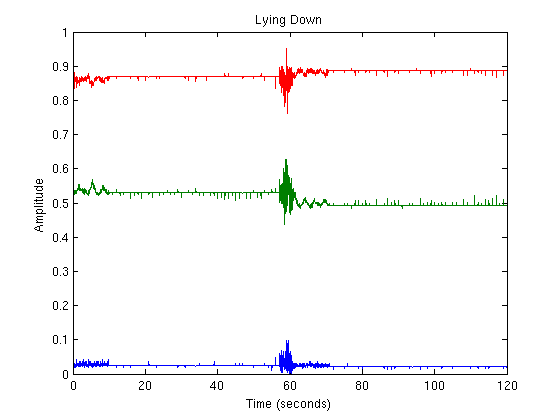
\includegraphics[scale=0.3]{osu_lying.png}
 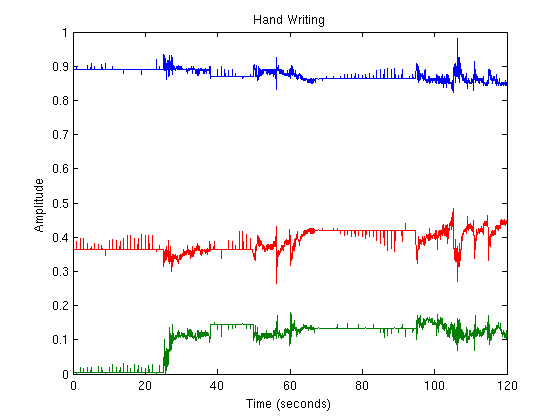
\includegraphics[scale=0.3]{osu_writing.png}
 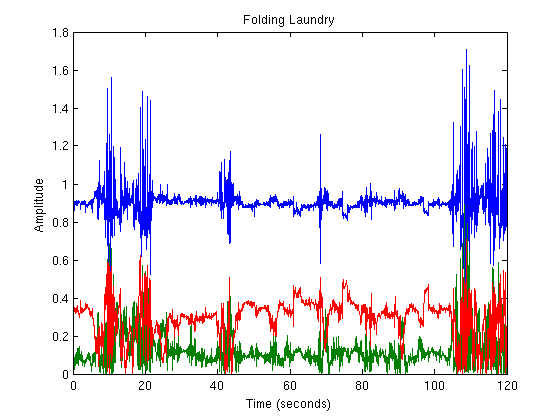
\includegraphics[scale=0.3]{osu_laundry.png}
 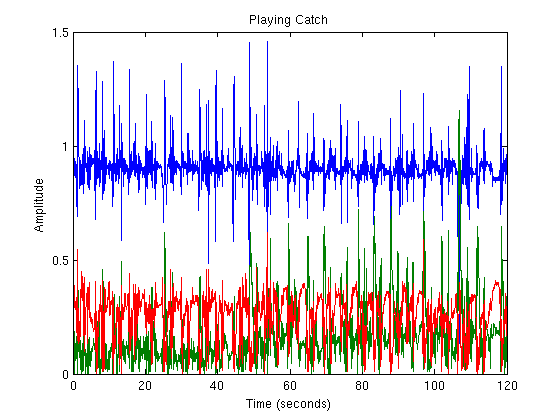
\includegraphics[scale=0.3]{osu_catch.png}
 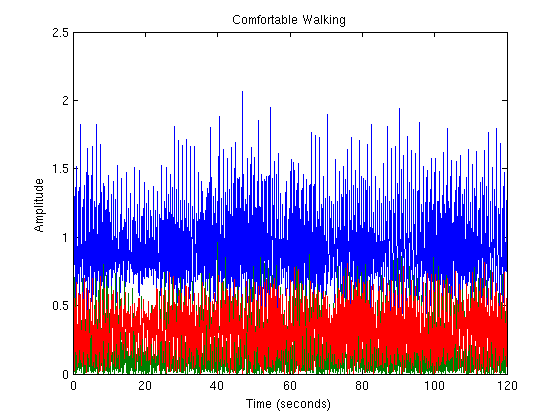
\includegraphics[scale=0.3]{osu_comf_walking.png}
 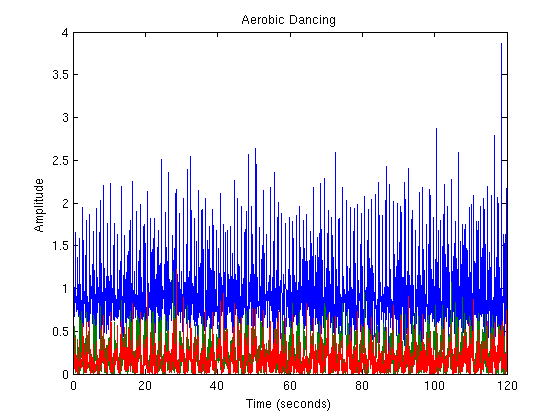
\includegraphics[scale=0.3]{osu_dancing.png}
 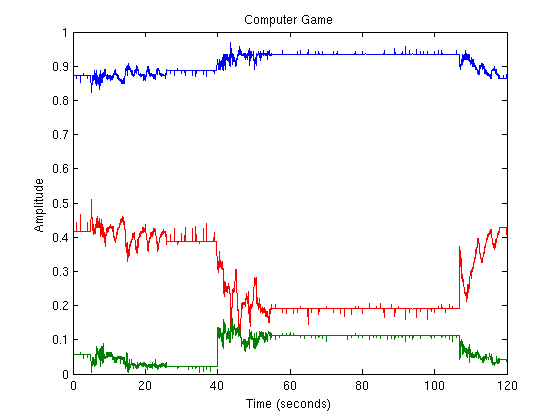
\includegraphics[scale=0.3]{osu_computer.png}
 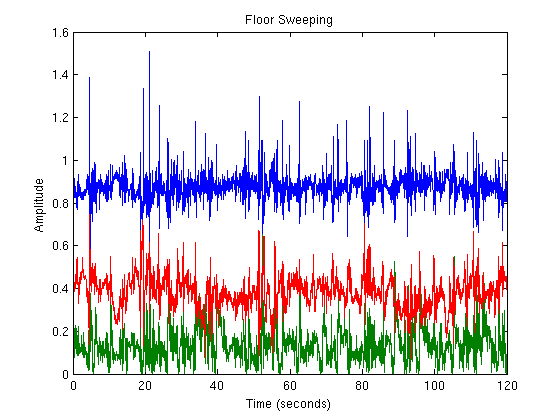
\includegraphics[scale=0.3]{osu_sweeping.png}
 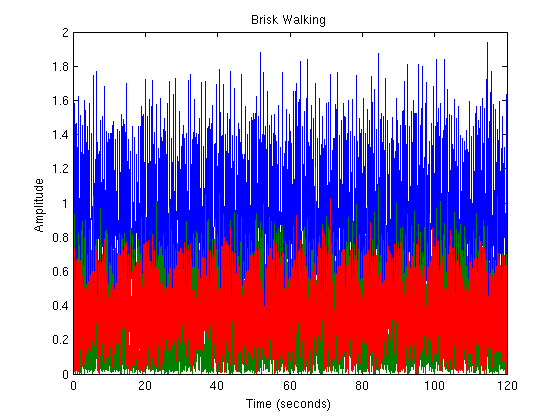
\includegraphics[scale=0.3]{osu_brisk_walking.png}
 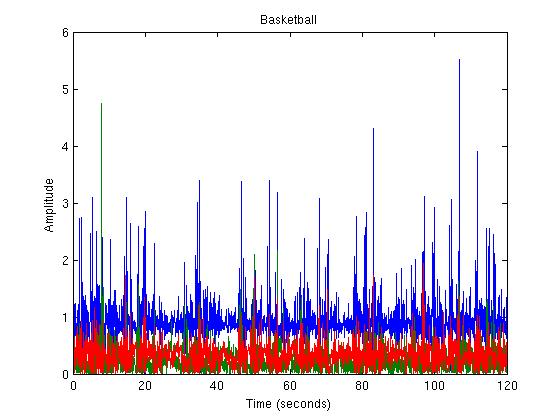
\includegraphics[scale=0.3]{osu_basketball.png}
 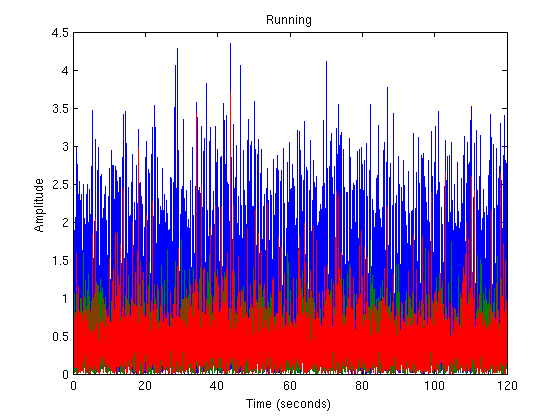
\includegraphics[scale=0.3]{osu_running.png}
 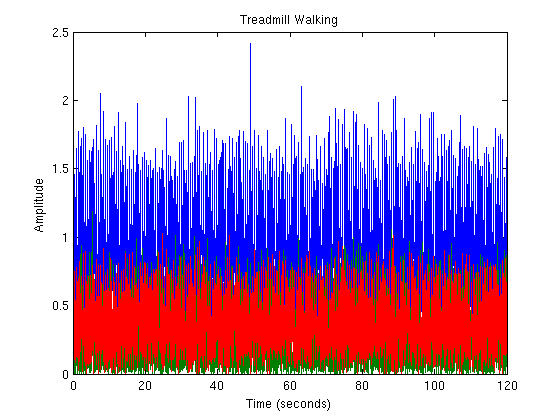
\includegraphics[scale=0.3]{osu_treadmill.png}
 \caption{OSU Hip Activity Samples}
 \label{fig:osu_activities}
\end{figure}

We determined that several of the activities were very similar and that
it would be difficult to discriminate between them, so we combined some of them together to
create a 7 class version of the data.
Our classes were lying down, sitting (hand-writing, computer game),
standing (laundry, sweeping, and catch), walking (comfortable, brisk and treadmill walking),
dancing, running, and basketball.

\subsection{UQ}
%TODO: Describe what research this data has been used for, and provide citation(s)

This dataset consisted of 23 time series, each containing roughly 10 continuous
days worth of data from a single subject. Subjects wore an ActiGraph GT3X+
accelerometer during the entire period, which collected triaxial acceleration data at a frequency
of 30Hz, as well as an activPal inclinometer on their thighs. The inclinometer
provided what we considered the ground truth labels of the data by automatically
delimitting and classifying intervals using the orientation of the subject's thigh at any given moment. It 
classified a horizontal orientation as lying down/sitting,
a vertical orientation as standing, and a combination of the two as walking. Figure
\ref{fig:uq_activities} shows samples of accelerometer data from the 3 activities.

\begin{figure}
 \centering
 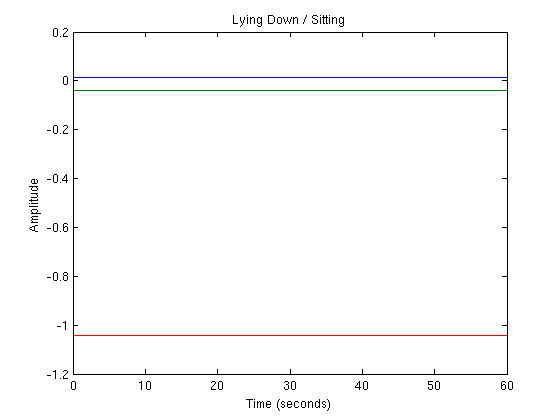
\includegraphics[scale=0.3]{uq_lying.png}
 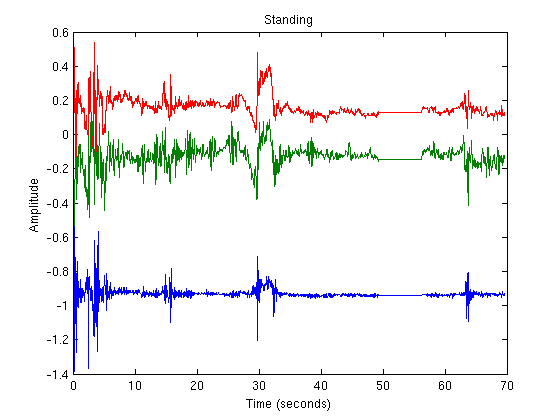
\includegraphics[scale=0.3]{uq_standing.png}
 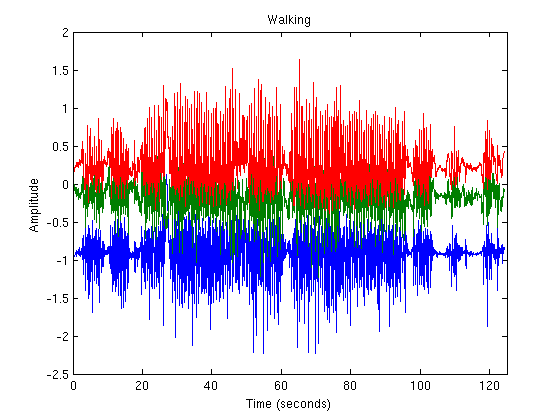
\includegraphics[scale=0.3]{uq_walking.png}
 \caption{UQ Day 1 Activity Samples}
 \label{fig:uq_activities}
\end{figure}

This dataset was challenging to work with because of its size, as each individual time series
contained roughly 25 million ticks of data. To help alleviate this problem, we split each
time series into individual days. We then treated the first day of data that began at midnight
from each subject as one whole dataset (UQ Day 1), and the second such day as a separate dataset
(UQ Day 2), and did not use the data from the remaining days.

%TODO: Number of events per time series, their mean and median size?

\section{Featurization}
To formulate our experiments as classification problems, we split each time series into a set of
non-overlapping windows and represented each window as a feature vector.
How we decided where one window ended (and where the next began) varied between
experiments, and is described in sections \ref{sec:topdown} and \ref{sec:bottomup}. Our feature
set was a large collection of statistics that have been shown to be discriminative
for activity classification in previous research \cite{li09} \cite{rothney07}
\cite{staudenmeyer09} \cite{zheng12}. In all we used 18 statistics that were
uniaxial, i.e. were only a function of the data from a single axis of a given window,
and one biaxial statistic.
The uniaxial statistics were applied to data from each axis separately, and
the biaxial statistic was applied to data from each of the $C_2^3=3$ possible pairs of
axes, for a total of $18*3+3 = 57$ features.

One discriminative characteristic of an activity is its overall vigorousness,
and the sum and the sample mean both act as simple and obvious ways of measuring this,
as more intense activities will tend to involve
higher rates of acceleration during movement. We also used the 10th, 25th (quartile 1),
50th (median), 75th (quartile 3), and 90th percentiles of the data, as well as signal
power and log energy as supplemental measures of overall activity intensity.

Another characteristic of an activity is how much it varies in intensity. The sample standard
deviation, coefficient of variation, peak-to-peak amplitude (max-min), zero crossings
(the number of times the data crosses its median), as well as the
interquartile range (75th\% - 25th\%) were useful for discriminating between activities
with a consistent level of intensity (low variance, etc.) and activities that were more
rhythmic or staccato in intensity (high variance, etc.). 

Skewness, kurtosis, lag-one-autocorrelation, and peak intensity
were useful for discriminating between
activities that tend to be similar in their overall intensity and variation in intensity,
but that showed other types of difference in shape. Skewness indicates whether the data is
more concentrated above or below its mean. Kurtosis indicates that the data is concentrated
near its mean or conversely that it is fat-tailed. Lag-one-autocorrelation is a measure of
the general relationship between data ticks and their immediate neighbors in time. Peak
intensity is the number of times that the data reached its maximum value. 

Finally we looked at a single bimodal statistic across each pair of axes, the correlation
coefficient, which discriminates between activities where acceleration values in one axis
are predictive of acceleration values in another axis, verses activities where that is not the case.

\section{Base Classifiers}

We tested 3 types of classification models on the featurized versions of our data:
decision trees, support vector machines, and neural networks. We used R for our
experiments, and used the `rpart', `e1071', and `nnet' libraries to R to build
our decision tree, svm, and neural net models, respectively. We treated the
decision tree as a simple and quick baseline algorithm, and did not tune it in
any way, ignoring the validation set. For all of the neural net experiments,
the maximum number of iterations was set to 100000, and the maximum number of
weights was set to 1000000.

For the OSU Hip experiments we tuned the
cost parameter $c$ of the svm on the validation set with 6 values:
$\{0.01,0.1,1,10,100,1000\}$. The single-layer feed-forward neural network took
two tuning parameters, and we tuned with each element of the set $H \times W$,
where $H = \{1,2, \ldots, 30\}$ was the numbers of nodes in the hidden layer, and 
$W = \{0,0.5,1\}$ was the weight decay parameters.

Since the UQ datasets were an order of magnitude larger, we tuned them
slightly differently because of time constraints. Setting the $c$ parameter to
1000 proved to be very computationally expensive for the svm model, so we tuned $c$
from the values $\{0.01,0.1,1,10,100\}$. Running $30*3=90$ tuning experiments
for the neural networks was also prohibitively expensive, so we drew from
$H \times W = \{5,10,15\} \times \{0,0.5,1\}$.

\section{Performance Metrics}
To measure the performance of our classification algorithms we used
two metrics. Accuracy is defined as the number of ticks that an algorithm
correctly classifies in a time series, over the total number of ticks
in the time series. Since we were also interested in our algorithms'
feasibility for activity classification in real time, we used detection time as
a second metric. Detection time is defined as the average amount of time
required for an algorithm to begin correctly classifying data after a
true activity change has occurred.

%TODO: Expand this section and/or include a picture.

\section{Top-Down Approach}
\label{sec:topdown}

\subsection{Change Point Detection}
For this approach, the data was split into non-overlapping segments for
featurization using techniques from the statistical field of change point detection.
Change point detection has found application in many problem domains that require analysis of time series data
from dynamic systems, including failure detection \cite{bae13}, quick detection of
attacks on computer networks \cite{tartakovsky06}, and monitoring of heartbeat fluctuations during
sleep \cite{staudacher05}. Change point detection assumes that each tick of a time series is a draw from some
process, but that the process may suddenly change as time passes.
The goal is to predict when these changes have occurred.
A \emph{score} is generated for each time tick, and if the score is
above a given threshold a change is predicted to have occurred between that tick
and its immediate predecessor. To generate a score at
a time tick, a window of data that immediately preceeds it (the
\emph{reference data}) is compared to it along with a window of data that immediately follows it
(the \emph{test data}).

\begin{figure}
 \centering
 \includegraphics[scale=0.8]{cpd_ref_test_new.png}
 \caption{Change Point Detection}
 \label{fig:cpd_ref_test.png}
\end{figure}

Model-based approaches to change point detection assume that each tick in
a time series is a draw from some underlying probability distribution.
Scores are generated by estimating the distribution of the reference data
and the test data, and then by calculating the likelihood
that the two distributions are different.
Where it is reasonable to assume that the data belongs to a particular
family of distributions then parametric estimation methods have been employed
\cite{thatte11}. If no such modeling assumptions are reasonable then 
non-parametric methods have also been found to be viable \cite{matteson12}.
Distance-based approaches such as Singular Spectrum Analysis
generate scores through other metrics of 
dissimilarity or difference between the reference data and the test data
\cite{moskvina03}.
Notationally, we say that for each tick $i$ in a time series:

\[
s_i = D(x_{r,i}, x_{t,i})
\]

Where $s_i$ is the score of the $i$th tick, $x_{r,i}$ is the reference
data associated with the $i$th tick, $x_{t,i}$ is the test data
associated with the $i$th tick, and $D(A,B)$ is a function that computes the
dissimiliarity between a matrix of data $A$ and matrix of data $B$, and varies
between change point algorithms. Note that for a given
algorithm it may not be possible to generate scores right at the very beginning
of the time series (insufficient reference data) or at the very end of a time
series (insufficient test data).

\subsection{Experimental Setup}

There are many different modeling assumptions and associated algorithms
for generating change point detection scores, and one simple baseline approach that we 
wanted to test was the Shewhart Control Chart. This approach assumes that the reference data is drawn from a
multivariate normal distribution, and that scores are calculated by the Mahalanobis
distance of the target time tick from the estimated multivariate normal:

\[
s_i = \sqrt{(\bar{x}_{r,i} - x_i)^T \, S_{r,i}^{-1} \, (\bar{x}_{r,i} - x_i)}
\]

where $\bar{x}_{r,i}$ is the sample mean of the reference data, $S_{r,i}$
is the sample covariance matrix of the reference data, and $x_i=x_{t,i}$ is
the $i$th data point \cite{shewhart26}.

We were also interested in testing the performance of a newer and more
sophisticated change point detection algorithm: the
Kullback-Leibler Importance Estimation Procedure (KLIEP),
introduced by Kawahara and Sugiyama \cite{sugiyama09} \cite{sugiyama08}.
This approach generates scores using the Kullback-Leibler (KL)
divergence between the reference data and the test data. One method of doing this
is to estimate the density of the reference distribution and test distribution
separately, and then compare them using a likelihood ratio
(known in the change point detection literature as \emph{importance}). 
Instead, KLIEP estimates the importance directly using a non-parametric model.

Let the estimate of the importance $\hat{R}$ be represented by this model:

\[
\hat{R} = \frac{p_{t}}{\hat{p}_{r}} = \sum_{j=1}^{n_{t}} \alpha_j K_G(x,x_{t,j})
\]

Where $p_{r}$ and $p_{t}$ are the probability densities of the reference data and the test
data, $n_{t}$ is the number of ticks in the test window, $\alpha$ is a
vector of model parameters to solve for, $x$ is the concatenation of the reference and the
test data, $x_{t,j}$ is the $j$th element of the test data,
and $K_G(A,B)$ is the Gaussian kernel with width $\sigma$:

\[
K_G(A,B) = \exp \left(-\frac{||A-B||^2}{2\sigma^2}\right)
\]

Now solve for $\alpha$ so that the empirical KL divergence between $\hat{p}_{t}$ and
$p_{t} = p_{r}\hat{R}$ is minimized, which is equivalent to the following convex optimization
problem:

\[
\begin{dcases}
 \max_{\alpha} \quad \sum_{j=1}^{n_t} \, \log \left( \sum_{k=1}^{n_t} \alpha_k K_G(x_{t,j}, x_{t,k}) \right) \\
 \,\, \text{s.t.} \quad\, \frac{1}{n_r} \sum_{j=1}^{n_r} \sum_{k=1}^{n_t} \alpha_k K_G(x_{r,j},x_{t,k}) = 1 \\
 \qquad \quad \text{and} \; \alpha_1 \ldots \alpha_{n_t} \ge 1
\end{dcases}
\]

Finally, the scores that we wish to generate are just the estimate of the importance given by the
solution to the complex optimization problem, i.e. $s_i = \hat{R}_i$.

Since this approach uses a Gaussian kernel, it requires the selection of
a kernel width $\sigma$ for each time tick. We used an implementation of
KLIEP that is available at Sugiyama's website, which included a cross-validation
procedure for the value of $\sigma$. The CV procedure chooses a number of disjoint
splits of the test data along with a number of different candidate $\sigma$'s, and runs
KLIEP with each combination of split and candidate $\sigma$. Then it chooses the candidate $\sigma$
that, on the average across all of the splits, maximizes the KL divergence (the
$\max_{\alpha}$ equation above) the most.

For the OSU Hip dataset, we used this CV procedure io choose the the kernel width at each individual time tick. This computationally
intensive approach was impractical for the UQ dataset because it is orders of magnitude larger,
so instead of running it on every tick of that data, we ran the CV procedure on a number of
random ticks drawn from the data. From this we were able
to empirically identify 0.01 as a plausible $\sigma$, and so fixed $\sigma$
at that value for our experiments on that dataset.

Previous research \cite{zheng12} found that on the average a window size of 10
seconds contained just enough information to discriminate well between OSU Hip activities.
Since this window size worked well in previous experiments, and since the 
activities of the UQ dataset were comparable in average length, we decided to
fix our reference window size at 10 seconds for both datasets. Because we were interested in
minimizing detection time, and because 1 second was the smallest window that
we felt could provide some information about an activity, we fixed our test
window size at 1 second for both datasets.

Once scores were generated, we tested a number of threshold values that determined which
scores were high enough to be considered a predicted change-point.
Threshold values were chosen by considering the false positive rates of
change prediction for the change point detection algorithms. A smaller false positive rate
corresponded to a higher and more conservative threshold, which split the
time series into fewer segments for featurization. A larger false positive rate
corresponded to a lower threshold, which split the time series into more segments.

\section{Bottom-Up Approach}
\label{sec:bottomup}

\subsection{HMMs}

Once we had created our methodology for splitting up time series using change-
point detection, we decided to test it against a more standard,
baseline technique. For this approach, we used the Hidden Markov Model to take
advantage of the sequential nature of our data. An HMM is a temporal graphical model
that contains a set of hidden states $H = \{H_0,H_1, \ldots, H_w\}$ as well as a set of
observed states $O = \{O_1,O_2, \ldots, O_w\}$ (Figure \ref{fig:hmm}). An index
of either type of state represents a point in time, such that if there exists
two indices $i$ and $j$ where $i < j$, $i$ is thought of as having happened
before $j$. Each hidden state in the model has one of a discrete set of values associated
with it drawn from $X=\{X_1,X_2, \ldots, X_{\ell}\}$, and each observed state has one
of a discrete set of values associated with it drawn from $Y=\{Y_1,Y_2, \ldots, Y_m\}$.
The values of the hidden states are unknown, and the values of the observable
states are known.
It is also assumed that, as indicated by Figure \ref{fig:hmm}, the
value of an observable state $O_i$ is dependent on the corresponding
hidden state $H_i$, and that the value of any hidden state $H_i$ is dependent only on
its immediate predecessor $H_{i-1}$.

Furthermore, the dependencies between hidden states and their followers are
assumed to be described by a stationary stochastic process known as the
\emph{transition model}, \mbox{$T: X^2 \rightarrow [0,1]$}. The dependencies
between a hidden state and its adjacent observable state are assumed to be part
of a separate but also stationary stochastic process known as the
\emph{observation model}, $S: X \times Y \rightarrow [0,1]$. In other words, both
models can be thought of as a function of two values, that output the
probability of a change from the first value to the second via a dependency
arc in the HMM. The usual approach to estimating $T$ and $S$ given only
$O$ is a flavor of expectation maximation known as the Baum-Welch algorithm,
which is useful for finding $\hat{T}$ and $\hat{S}$ that are locally maximally
likely. However, suppose a \emph{training HMM} $\langle H_{tr},O_{tr} \rangle$
with the same model parameters is given, and the values of all of its hidden states as well as its
observable states are known. $T$ and $S$ are then approximated by the
following global maximum likelihood estimators:

\[
\hat{T}(X_i,X_j) = \frac{|\{H_k \in H_{tr} \; | \; H_k=X_i \; \text{and} \; H_{k+1}=X_j\}|} {|\{H_k \in H_{tr} \; | \; H_k=X_i\}|}
\]

\[
\hat{S}(X_i,Y_j) = \frac{|\{H_k \in H \; | \; H_k=X_i \; \text{and} \; O_k=Y_j\}|} {|\{H_k \in H \; | \; H_k=X_i\}|}
\]

\begin{figure}
 \centering
 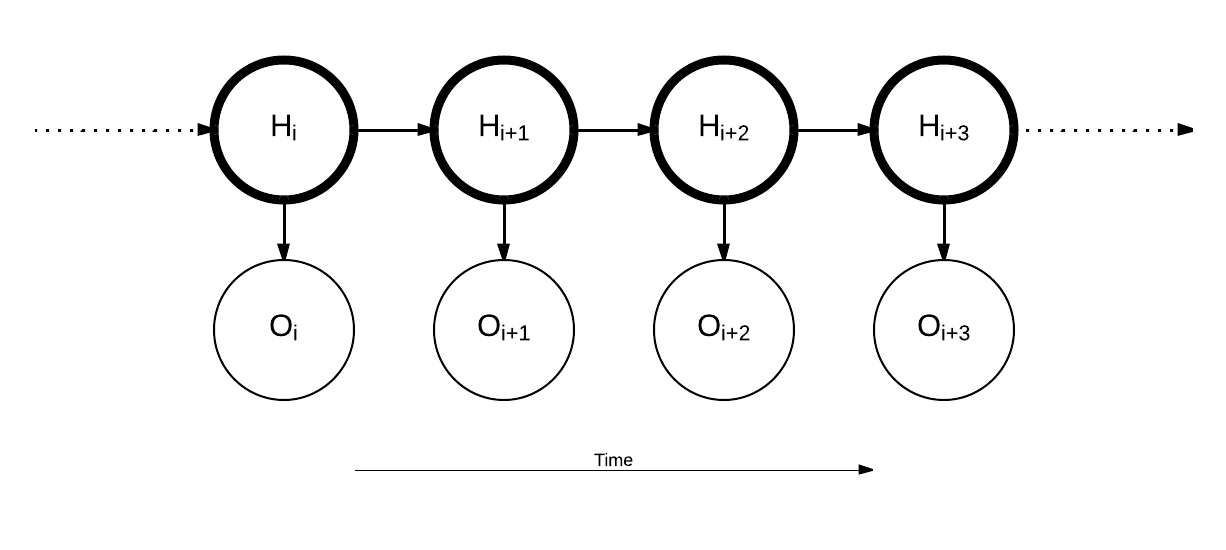
\includegraphics[scale=0.3]{hmm.png}
 \caption{Visual Interpretation of an HMM}
 \label{fig:hmm}
\end{figure}

Finally, if all of the values of $O$ are known, and we are given
a $\hat{T}$ and an $\hat{S}$ estimated from a training HMM, then the goal we are interested in
is to use that information (along with the model assumptions)
to find the most likely values for each state in $H$. There
exists a polynomial-time dynamic programming solution to this problem known as
the Viterbi algorithm. \cite{russell10}

\subsection{Experimental Setup}

For our experiments we began by splitting each time series into small non-overlapping windows. Within a
given experiment the window size was fixed, but across different experiments we
tested window sizes of length $\{1,2, \ldots ,20\}$. Once the time series were
split they were featurized. Classification
models were built with training data,
and tuned (in the case of the svm and neural net models) using validation data,
in the same way that has already been described previously in this chapter.

Unlike the change-point detection experiments, this experiment required
that the data be split into 4 equal parts: training (classifier), validation,
training (HMM), and testing) rather than 3. 
Here we formulated the problem of making predictions on the testing set in terms
of an HMM, first by treating the second training set as a training HMM. Each
window of the second training set was treated as a time index ${1,2, \ldots, n}$.
In our datasets we
let $H$ be the ground truth activity classes of the windows, and $O$ be the
predicted activity classes of the windows. We used the precedure above to
calculate $\hat{T}$ and $\hat{S}$, and assumed that these estimates held for
the testing set as well as the second training set. We then used the
tuned base classifier to predict on the testing set, giving us $O$. Finally,
we used $O$, $\hat{T}$, and $\hat{S}$ to run the Viterbi algorithm on the
testing set and predict the ground truth activity classes $H$.


\chapter{Results}
%Figure \ref{fig:cpd_perf}, shows accuracy and detection time as a function of the
%false positive rate per second, for the OSU Hip dataset,
%for each of the SVM, Decision Tree, and Neural Net base classifiers.
%
%\begin{figure}
% \centering
% 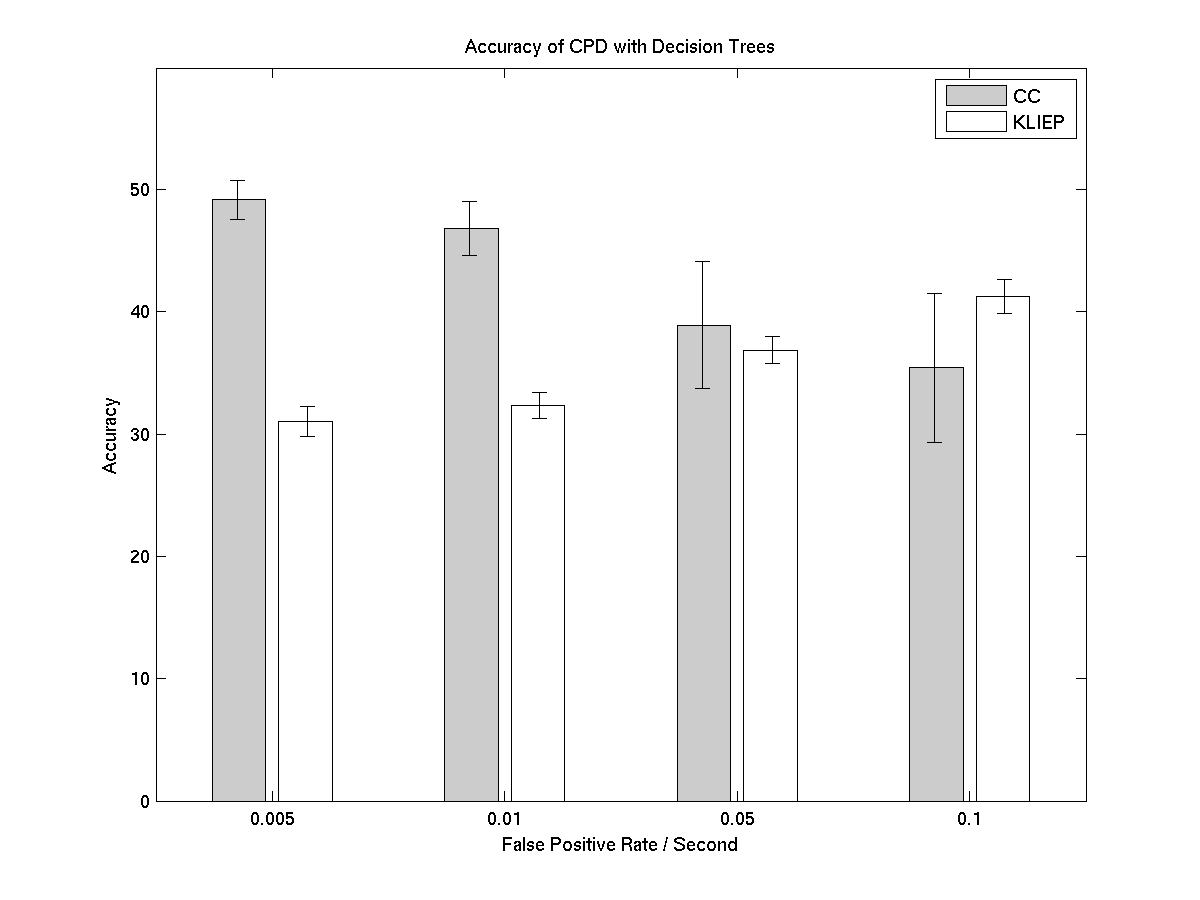
\includegraphics[scale=0.3]{osu_cpd_dt_acc.png}
% 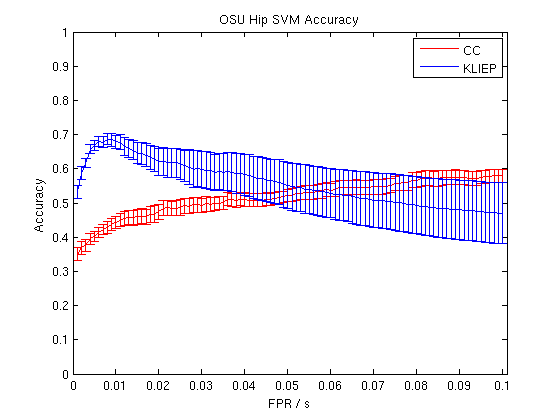
\includegraphics[scale=0.3]{osu_cpd_svm_acc.png}
% 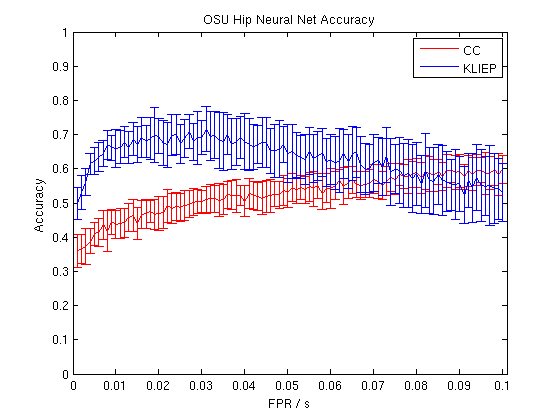
\includegraphics[scale=0.3]{osu_cpd_nnet_acc.png}
% 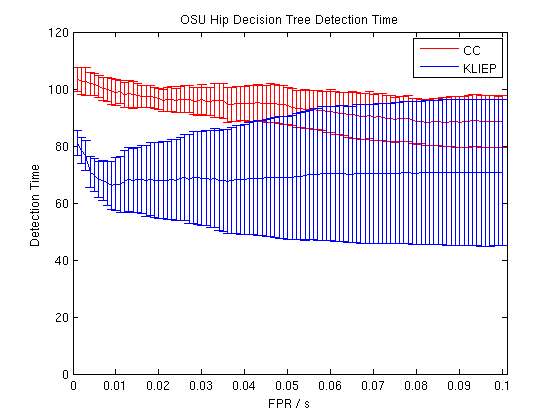
\includegraphics[scale=0.3]{osu_cpd_dt_det.png}
% 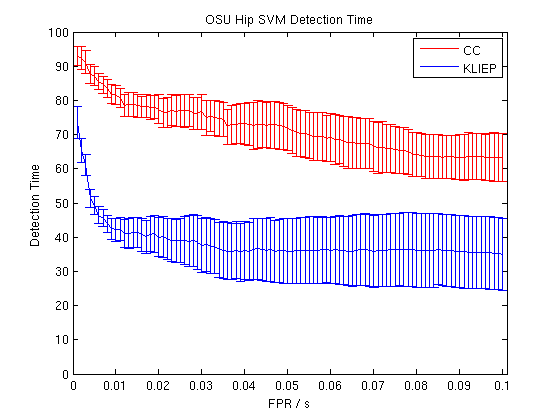
\includegraphics[scale=0.3]{osu_cpd_svm_det.png}
% 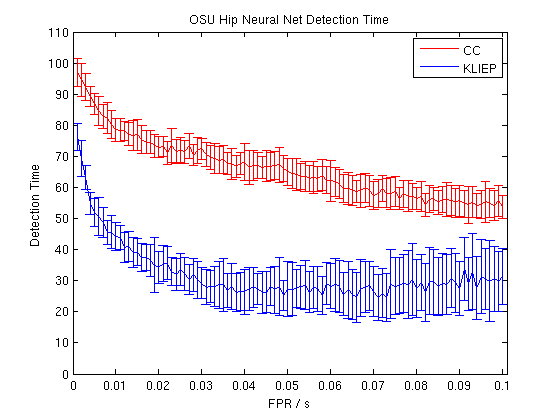
\includegraphics[scale=0.3]{osu_cpd_nnet_det.png}
% \caption{CPD-Based Classification Performance}
% \label{fig:cpd_perf}
%\end{figure}

\section{Top-Down}
\label{sec:cpd_results}

Results for our change-point detection experiments are given in
Figures \ref{fig:osu_cpd}-\ref{fig:lime2_cpd}.
The performance of the change-point detection algorithms
depended heavily on the threshold level for change prediction. In our
experiment we varied the threshold level, thus changing the false positive
rate. A large number of false positives per
second were tested, but for the sake of brevity only a representative sample
of $\{0.005, 0.01, 0.05, 0.1\}$ are shown here.

In the OSU Hip experiments, control charts outperformed KLIEP in terms of
detection time (Figures 4.1.2, 4.1.4, 4.1.6), while the accuracy results 
(Figures 4.1.1, 4.1.3, 4.1.5) were
mixed. Except when predicted windows are large enough to span across multiple
true activities, it is generally expected that accuracy will decrease as false
positive rate increases because small windows contain less information and are
less discriminative than larger windows. This behavior is seen in the control chart
accuracy results (grey bars in Figures 4.1.1, 4.1.3, 4.1.5), but not in the
KLIEP accuracy results (white bars in Figures 4.1.1, 4.1.3, 4.1.5).
Follow-up experiments showed that KLIEP peaks in accuracy for
false positives per second between $0.2$ and $0.3$ for all three classifiers.
KlIEP seemed to perform best on this dataset when it was given many
opportunities to predict changes.

Further investigation indicated that across the OSU Hip dataset the KLIEP algorithm
was unable to detect many of the different activity changes without a very low score
threshold value (and a very high false positive rates).
Some qualitative plotting of the OSU Hip data showed
that most of its activities have accelerometer amplitude values that strongly
resemble draws from a multivariate normal distribution. Since control charts
assume that the data is drawn from a distribution that is a member of that
family, it is logical that control charts would outperform algorithms with
different modeling assumptions on OSU Hip.

In the LiME experiments, KLIEP outperformed control charts in terms of
accuracy across the board, and control charts outperformed KLIEP in terms of
detection time across the board. This suggests that in general control charts
correctly detected true changes more quickly, but that after a correct change
prediction it was more likely to make an incorrect change prediction.

In a few cases (Figures 4.1.2, 4.1.6, 4.2.6) the detection time did
not decrease as the false positive rate increased. On the face of it this would seem
to be a non-sequitur, but this only happened in cases when accuracy also decreased
(Figures 4.1.1, 4.1.5, 4.2.5).
Smaller window sizes tend to be correlated with decreased detection times, but
it is possible that predicting with smaller windows, if they happen to contain
an insufficient amount of discriminative data,
can actually increase the time required for the classifier to start correctly
predicting the ground-truth activity. Additionally, the given increases in detection
time were small and within confidence bounds.

\begin{figure}[H]
 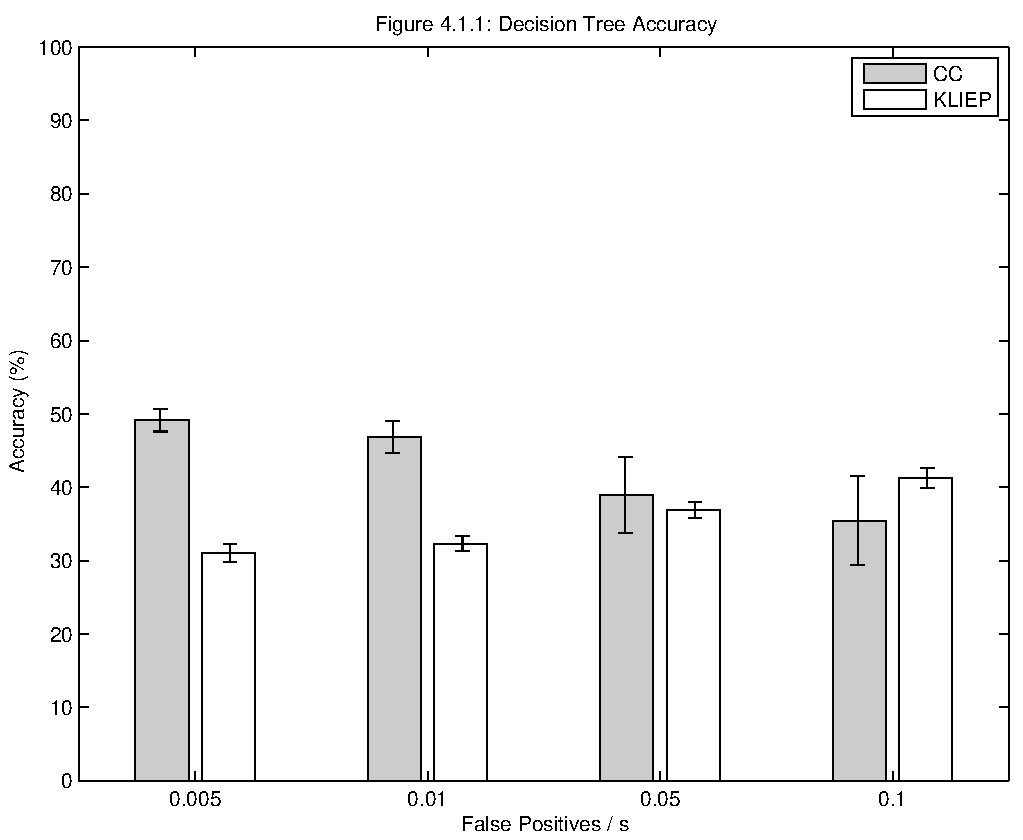
\includegraphics[scale=0.4]{osu_cpd_dt_acc.pdf} \hspace{1em}\vspace{1em}
 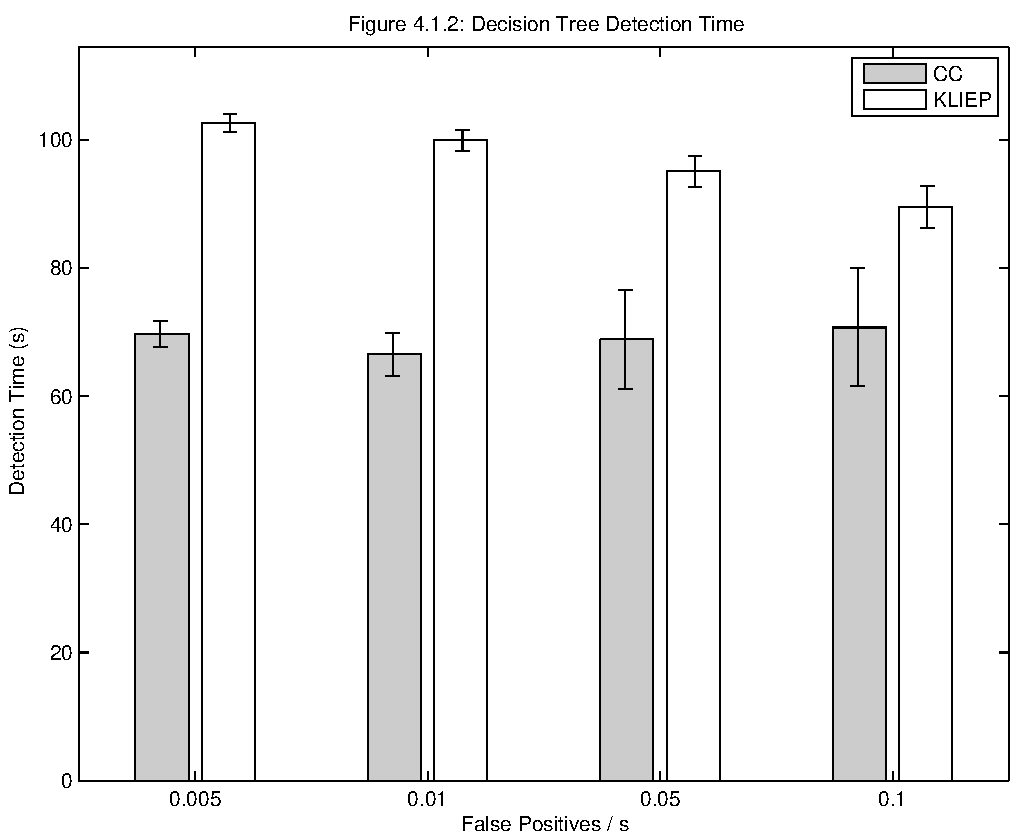
\includegraphics[scale=0.4]{osu_cpd_dt_det.pdf}
 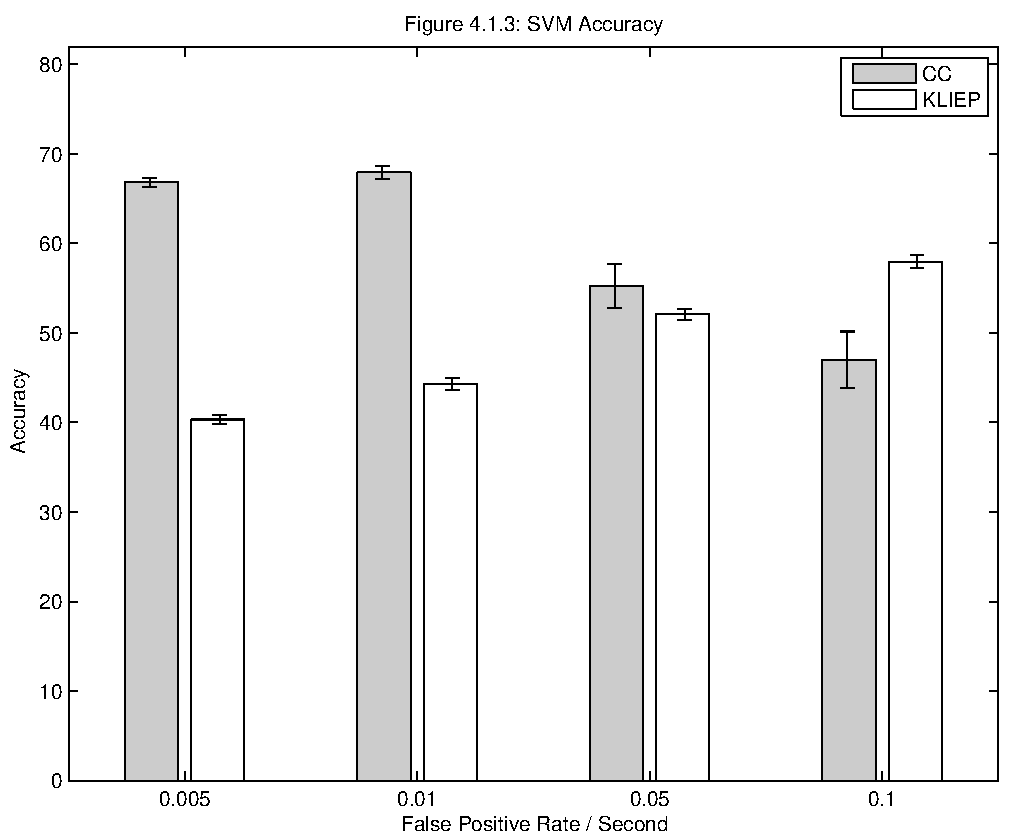
\includegraphics[scale=0.4]{osu_cpd_svm_acc.pdf} \hspace{1em}\vspace{1em}
 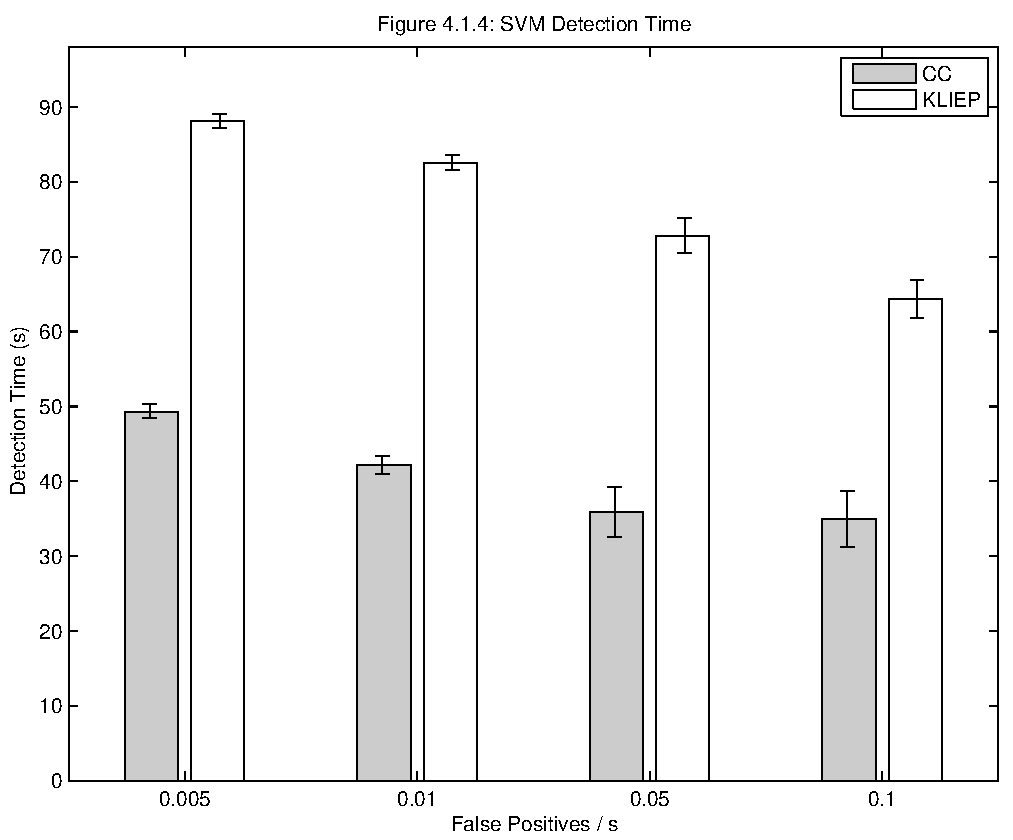
\includegraphics[scale=0.4]{osu_cpd_svm_det.pdf}
 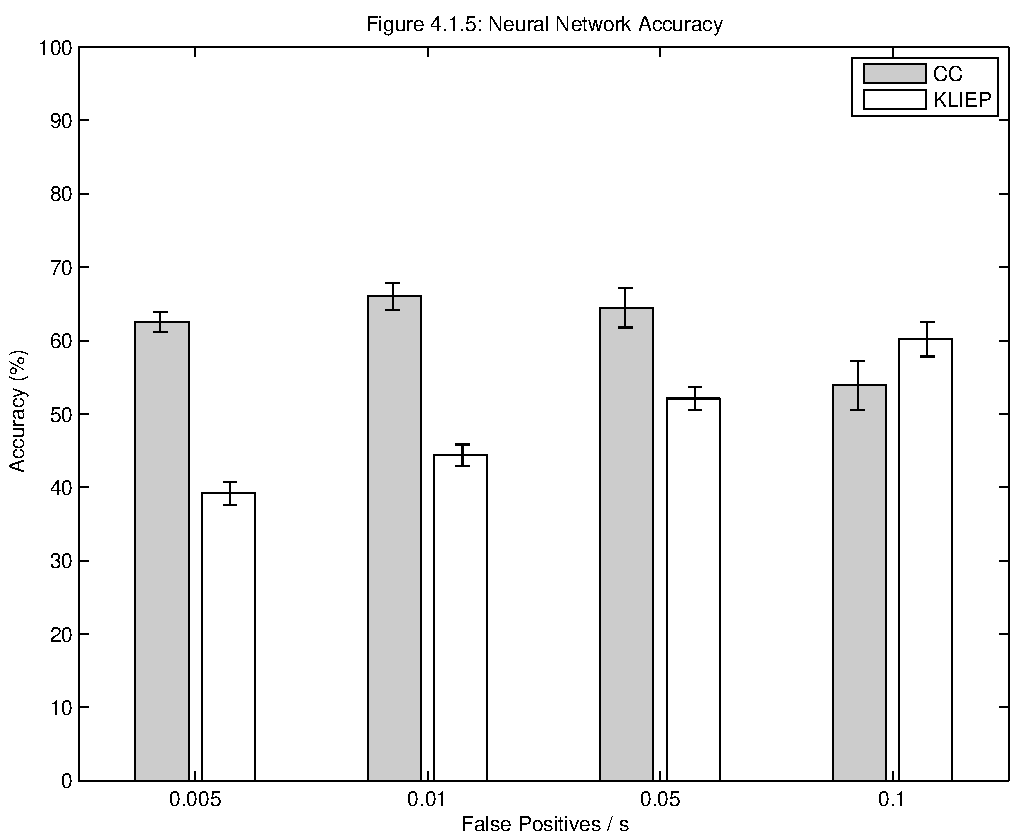
\includegraphics[scale=0.4]{osu_cpd_nnet_acc.pdf} \hspace{2em}
 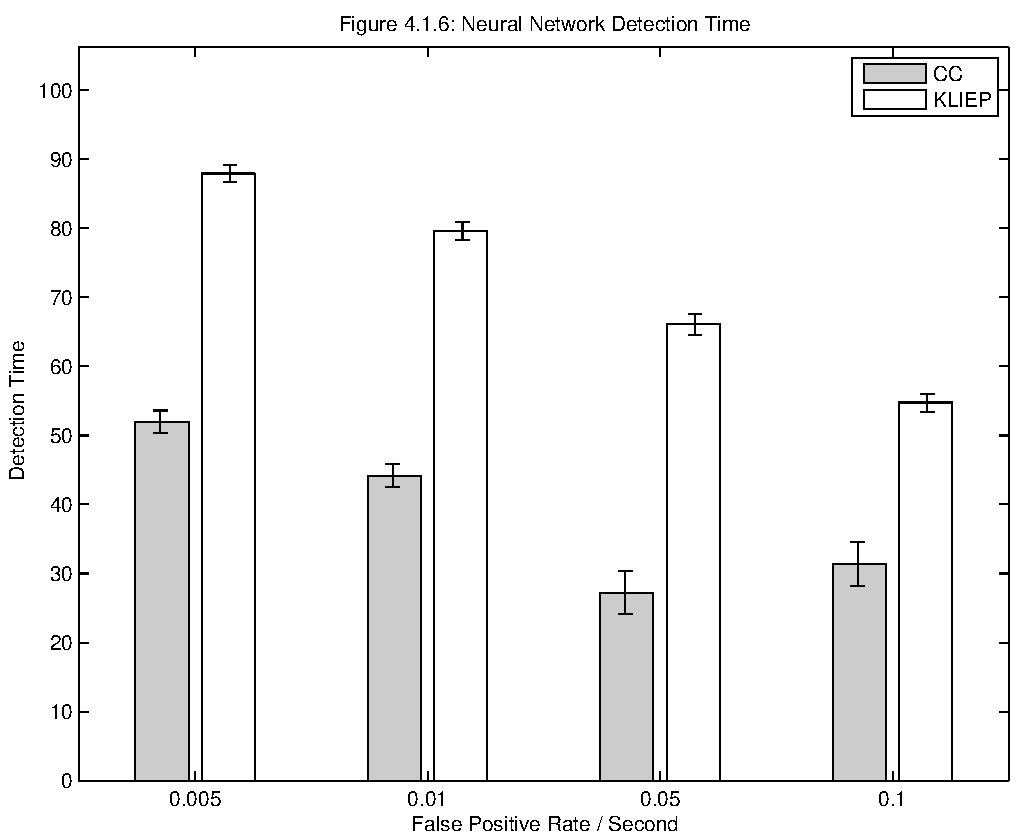
\includegraphics[scale=0.4]{osu_cpd_nnet_det.pdf}
 \caption{OSU Hip Results. Graphs are organized into rows by base classifier,
  and columns by evaluation metric. Change-point detection results were averaged over
  30 splits into training, testing, and validation datasets. Error bars show a
  95\% confidence interval around the average.}
 \label{fig:osu_cpd}
\end{figure}

\begin{figure}[H]
 \centering
 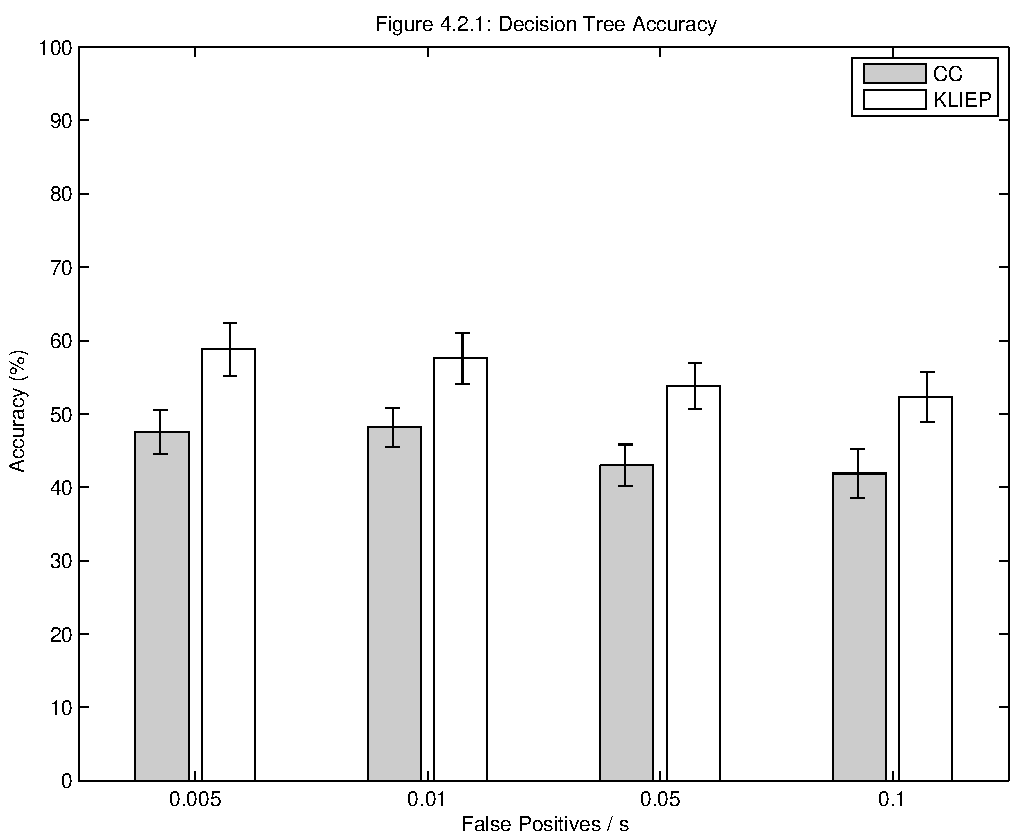
\includegraphics[scale=0.4]{lime1_cpd_dt_acc.pdf} \hspace{1em}\vspace{1em}
 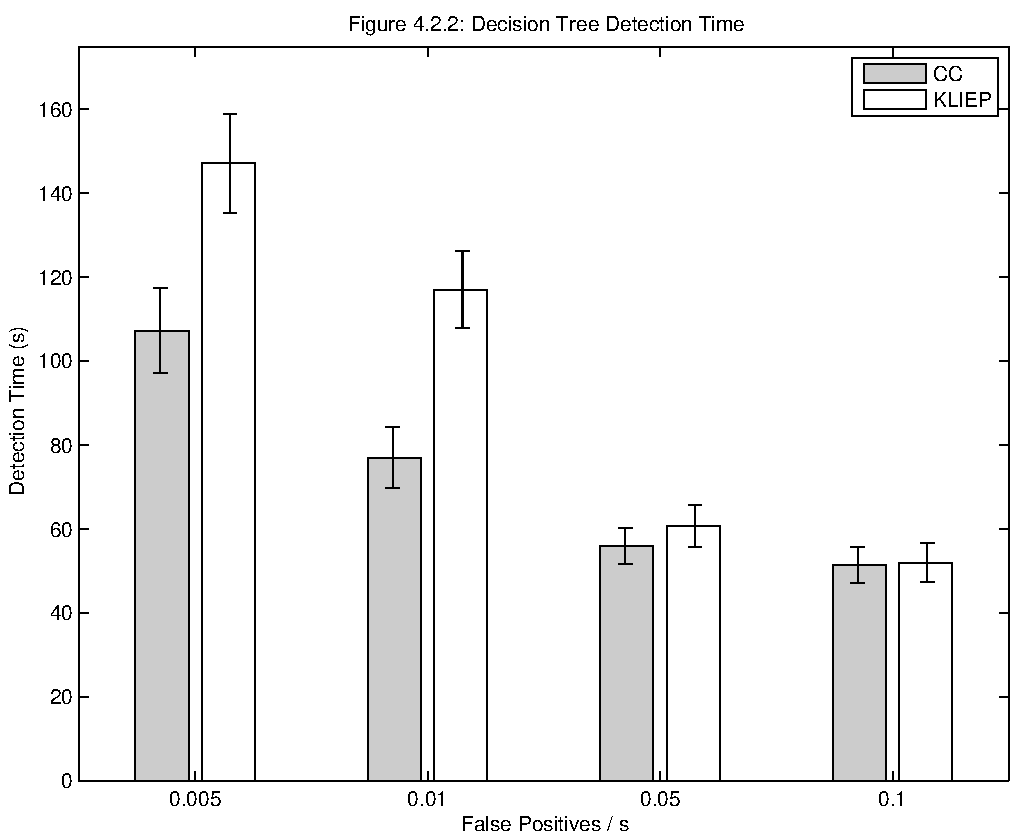
\includegraphics[scale=0.4]{lime1_cpd_dt_det.pdf}
 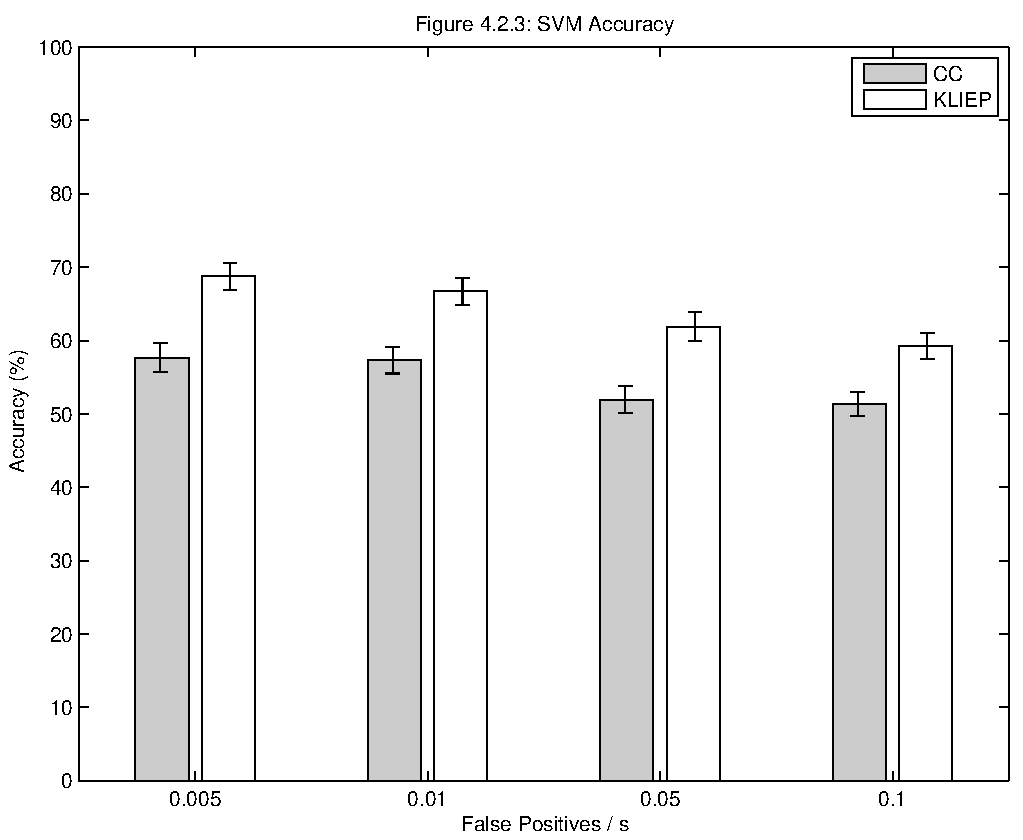
\includegraphics[scale=0.4]{lime1_cpd_svm_acc.pdf} \hspace{1em}\vspace{1em}
 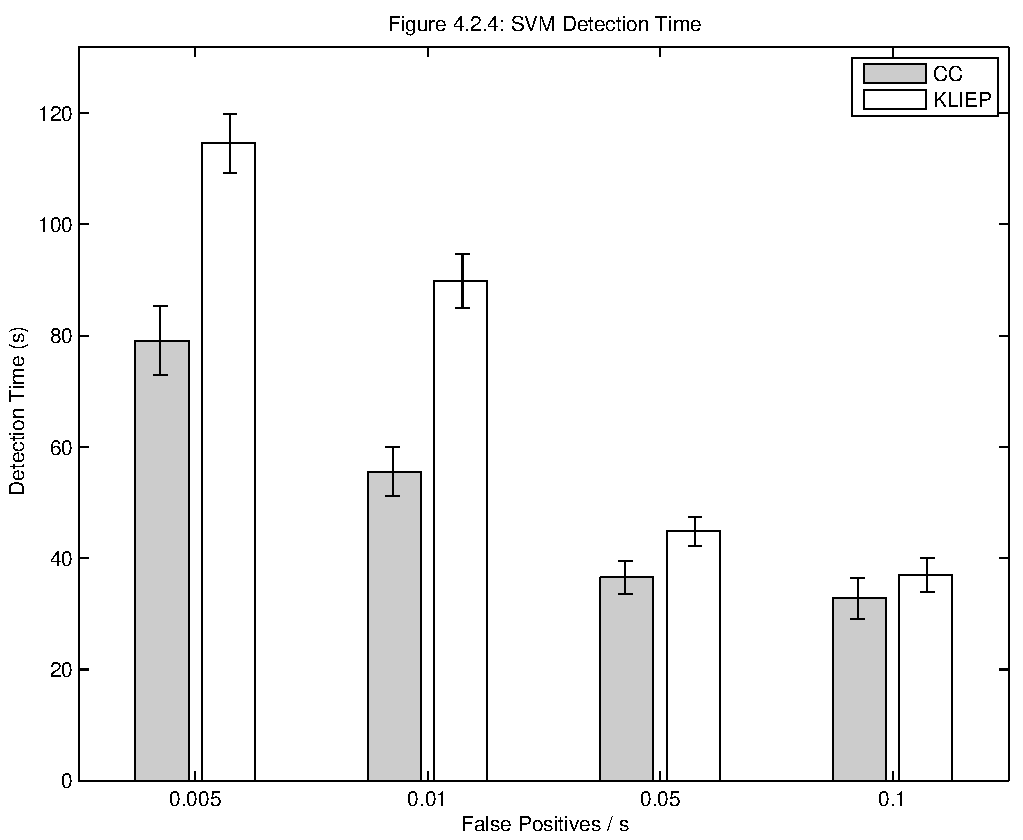
\includegraphics[scale=0.4]{lime1_cpd_svm_det.pdf}
 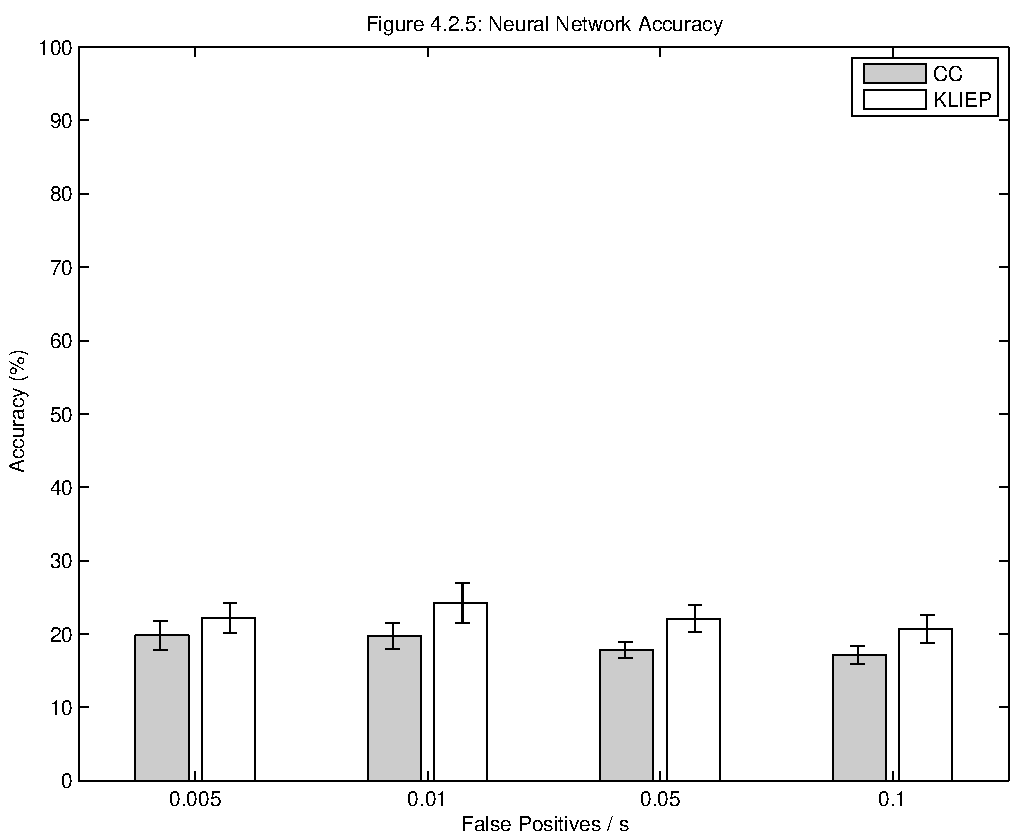
\includegraphics[scale=0.4]{lime1_cpd_nnet_acc.pdf} \hspace{1em}
 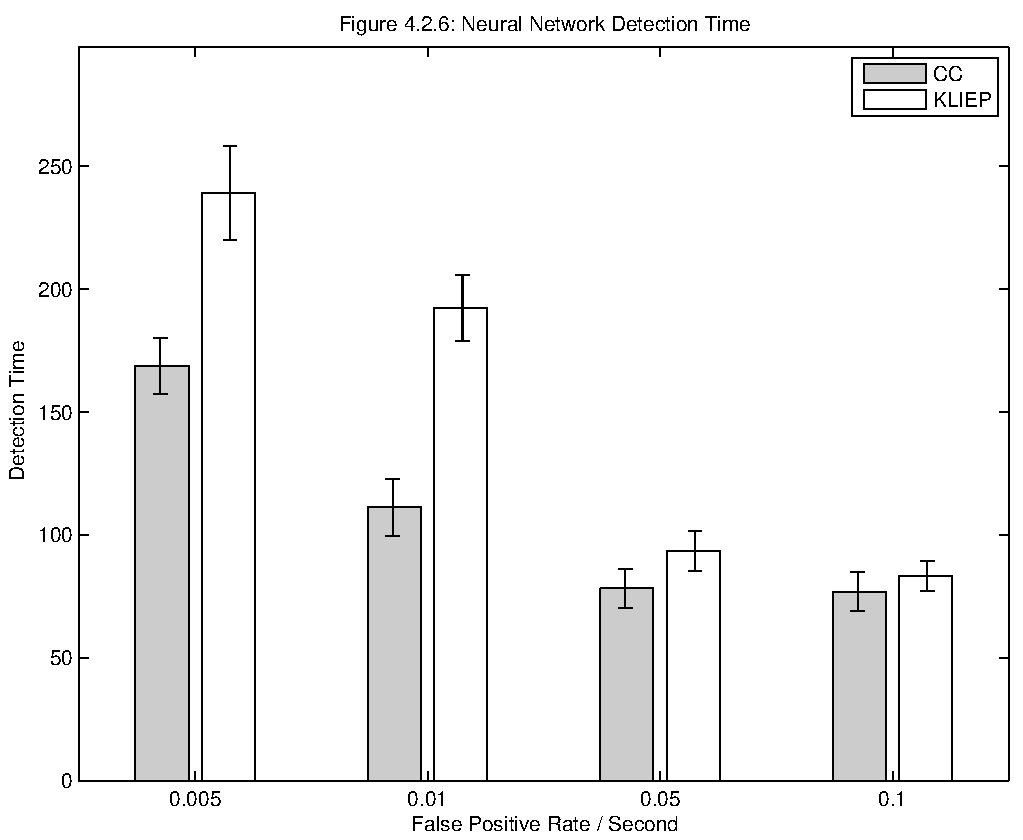
\includegraphics[scale=0.4]{lime1_cpd_nnet_det.pdf}
 \caption{LiME Day 1 Results. Graphs are organized into rows by base classifier,
  and columns by evaluation metric. Change-point detection results were averaged over
  30 splits into training, testing, and validation datasets. Error bars show a
  95\% confidence interval around the average.}
 \label{fig:lime1_cpd}
\end{figure}

\begin{figure}[H]
 \centering
 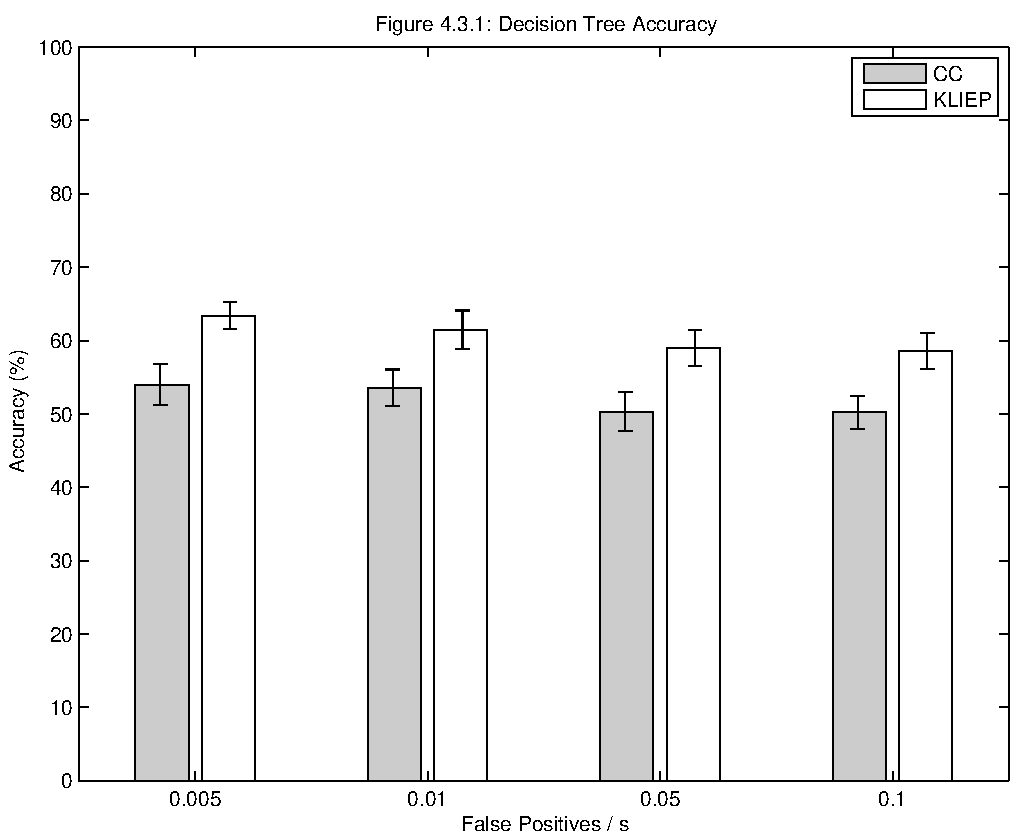
\includegraphics[scale=0.4]{lime2_cpd_dt_acc.pdf} \hspace{1em}\vspace{1em}
 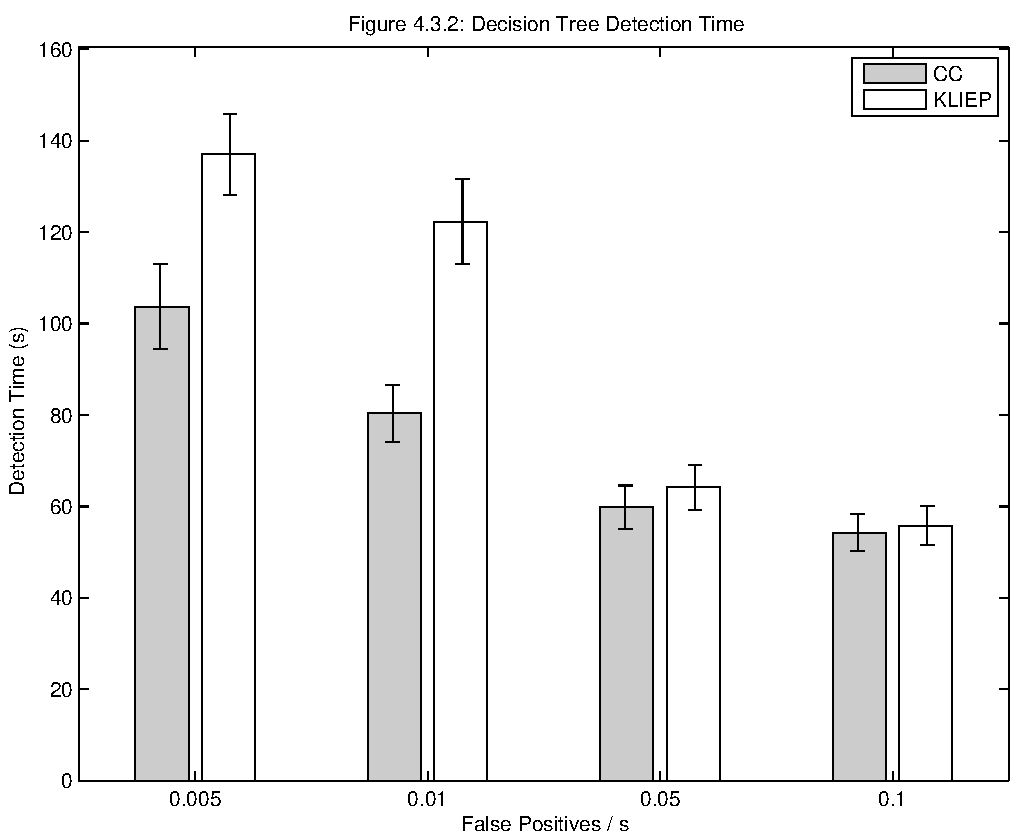
\includegraphics[scale=0.4]{lime2_cpd_dt_det.pdf}
 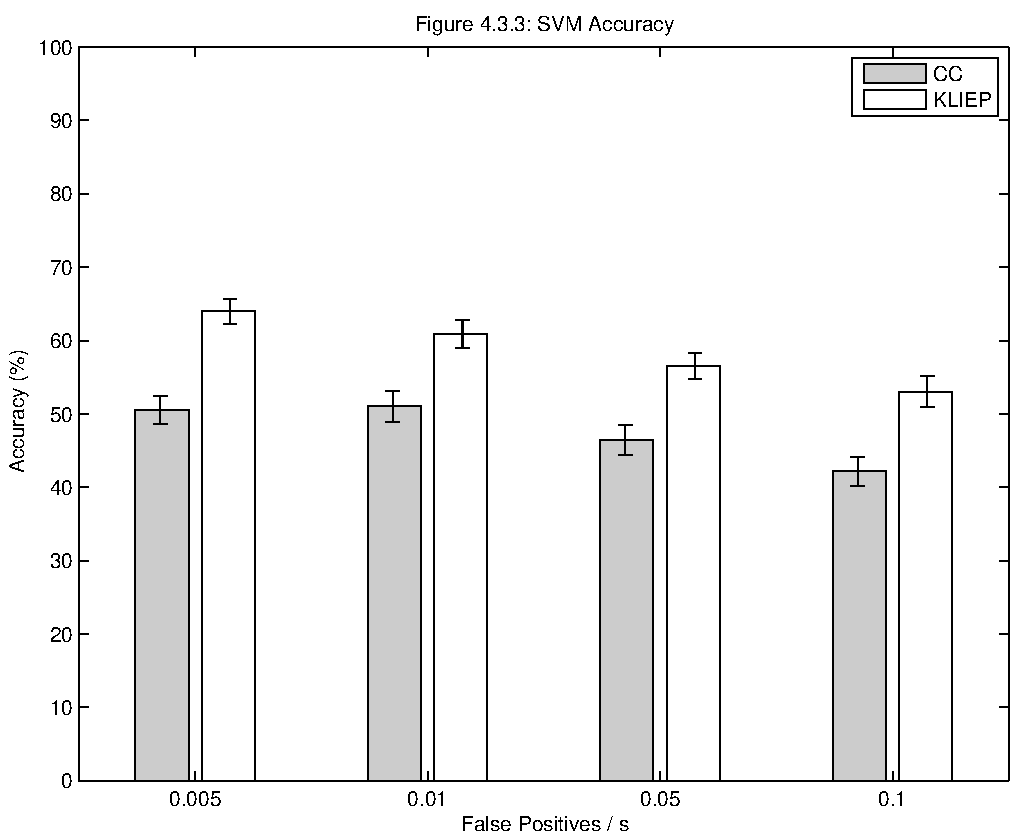
\includegraphics[scale=0.4]{lime2_cpd_svm_acc.pdf} \hspace{1em}\vspace{1em}
 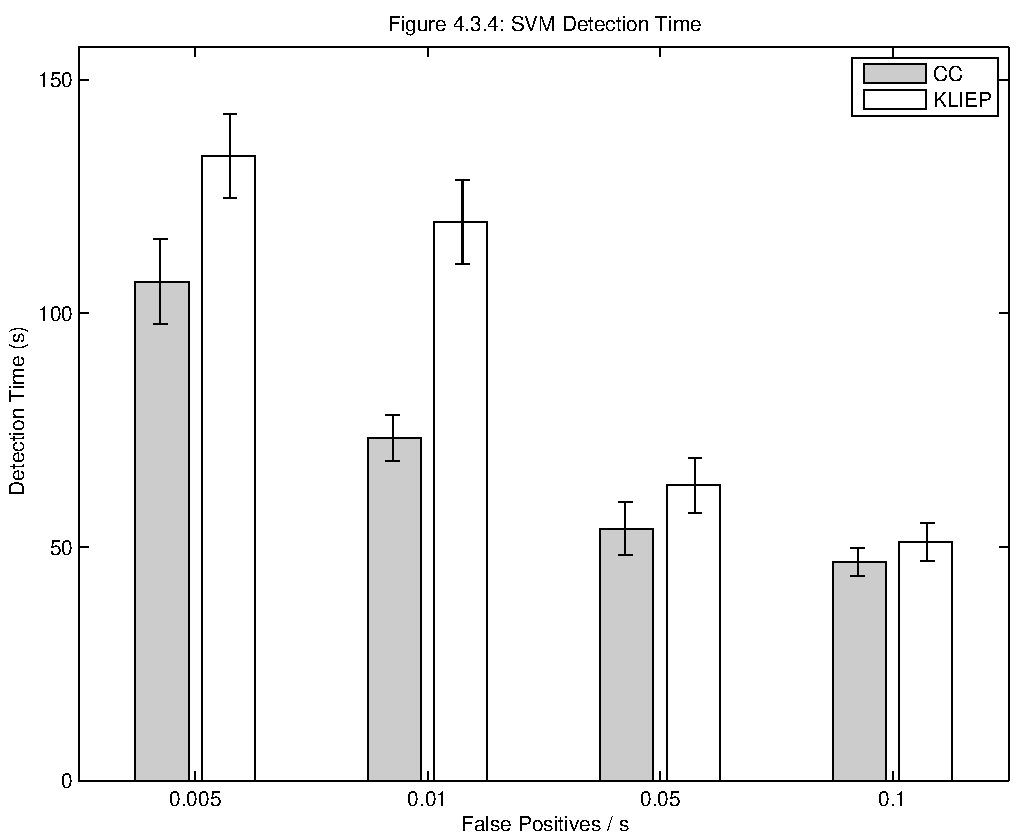
\includegraphics[scale=0.4]{lime2_cpd_svm_det.pdf}
 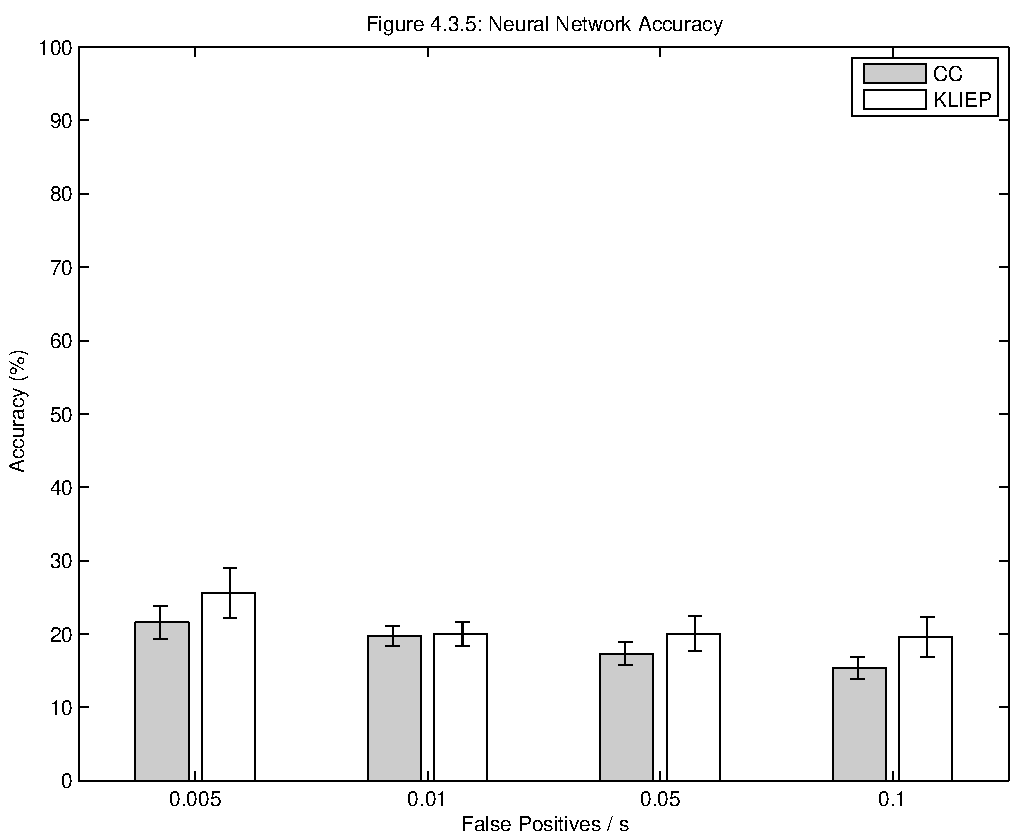
\includegraphics[scale=0.4]{lime2_cpd_nnet_acc.pdf} \hspace{1em}
 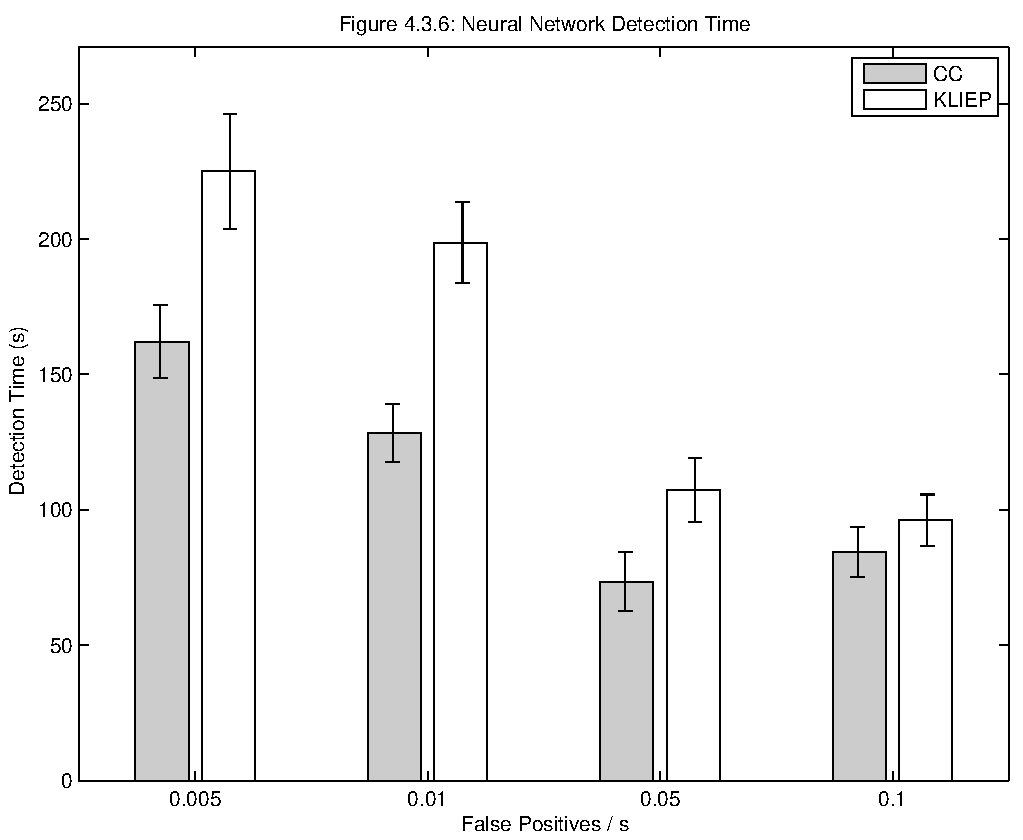
\includegraphics[scale=0.4]{lime2_cpd_nnet_det.pdf}
 \caption{LiME Day 2 Results. Graphs are organized into rows by base classifier,
  and columns by evaluation metric. Change-point detection results were averaged over
  30 splits into training, testing, and validation datasets. Error bars show a
  95\% confidence interval around the average.}
 \label{fig:lime2_cpd}
\end{figure}


\section{Bottom-Up}

Results for our bottom-up experiments are given in
Figures \ref{fig:osu_hmm}-\ref{fig:lime2_hmm}. Each experiment was
performed by splitting each time series into windows of fixed length
corresponding to discrete time ``ticks'' in an HMM,
and results for windows of length $\{10, 12, 14, 16, 18, 20\}$
seconds are shown.

For all three base classifiers, accuracy was high and
stable with respect to window size, over all three datasets. Detection
time was also fairly stable in the OSU Hip experiments, though as would
generally be expected it increased somewhat with window size in the LiME
experiments. Further experiments [results not shown] on the
OSU Hip dataset showed that the accuracy and detection time of our bottom-up approach 
tends to be poor for very small window sizes, but that it stabilizes with window sizes
that are greater than roughly 5 seconds. This gives a strong indication that
5 seconds is the amount of information necessary for the classifiers to become as
discriminative as they can be on the datasets in our work.

Using the HMM tended to give a slight boost in accuracy to the base classifiers,
but at the expense of increased detection time. It is likely that the increase
in accuracy was due to the smoothing of false base classifier predictions that
were sandwiched in time between true base classifier predictions, and that the increase in
detection time was due to the general stickyness of activities. Once the
subject started performing an activity the probability of the subject stopping
that activity to start a new one was recognized to be low, which meant that a true change in
activities would be unlikely to be recognized by the smoothing algorithm
immediately.

The experiments also show the reason for the difference in
performance between the top-down and bottom-up approaches. 
The difference could have been caused by the
use of change-point detection algorithms to segment the data as opposed to using
fixed length windows, or the ability of the HMM
to smooth predictions made on temporal data. The side-by-side comparison of the
same fixed window length classification experiments performed with and without HMM smoothing
suggests that the smoothing effect of the HMM
does not explain most of the performance difference, and that the performance difference between the top-down
and bottom-up approaches was mostly due to noisy segmentation by the change-point
detection algorithms.

 
\begin{figure}[H]
 \centering
 %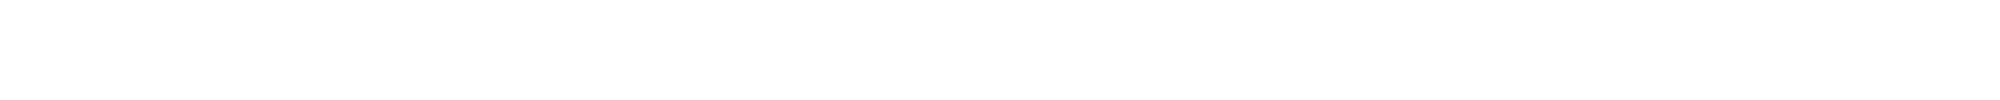
\includegraphics[scale=0.3]{vspace.png}
 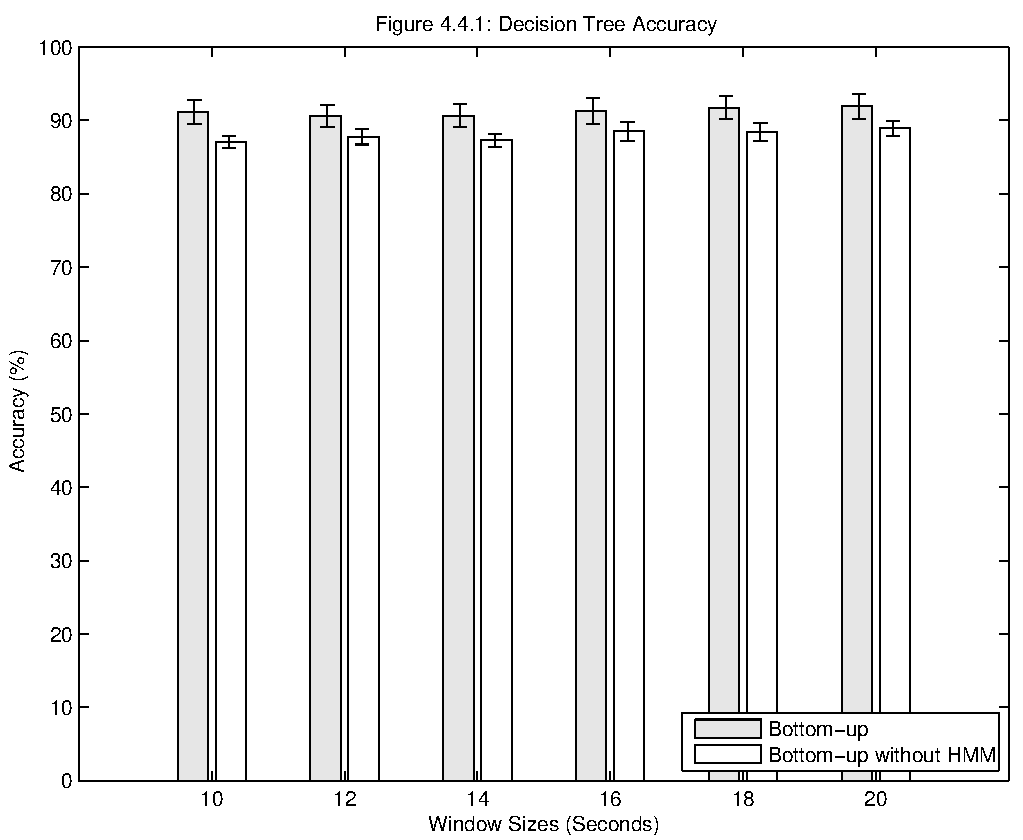
\includegraphics[scale=0.4]{osu_dt_hmm_nohmm_compare_acc.pdf} \hspace{1em}\vspace{1em}
 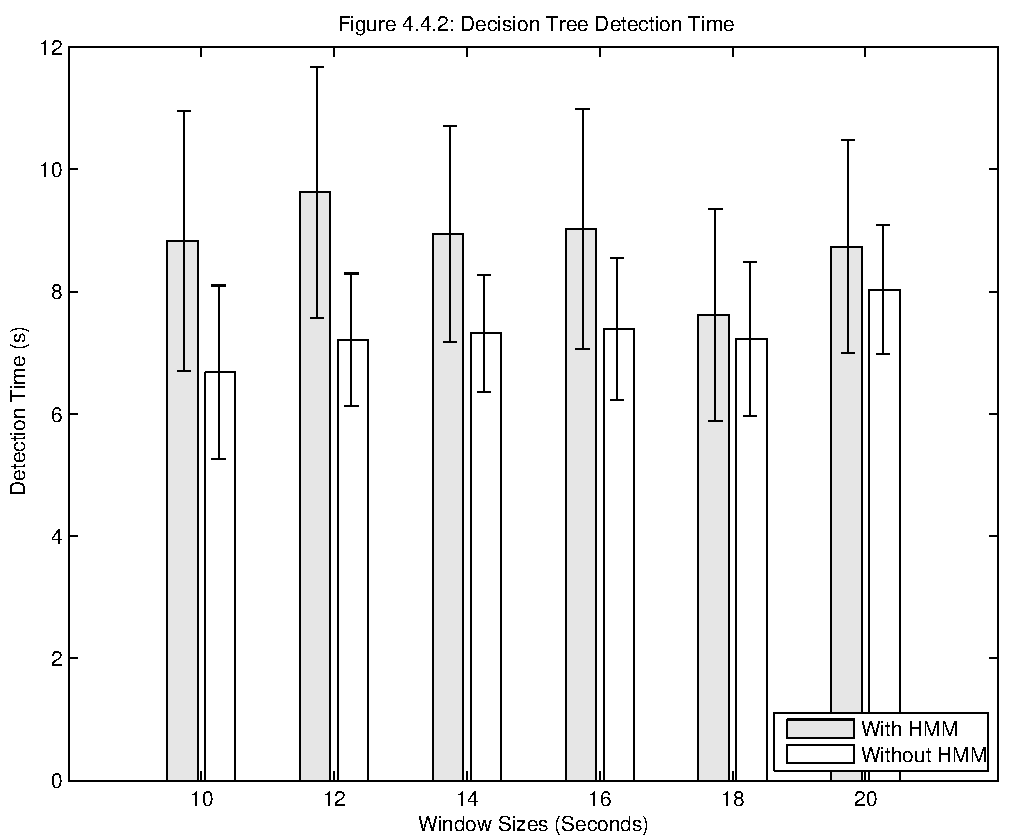
\includegraphics[scale=0.4]{osu_dt_hmm_nohmm_compare_det.pdf} 
 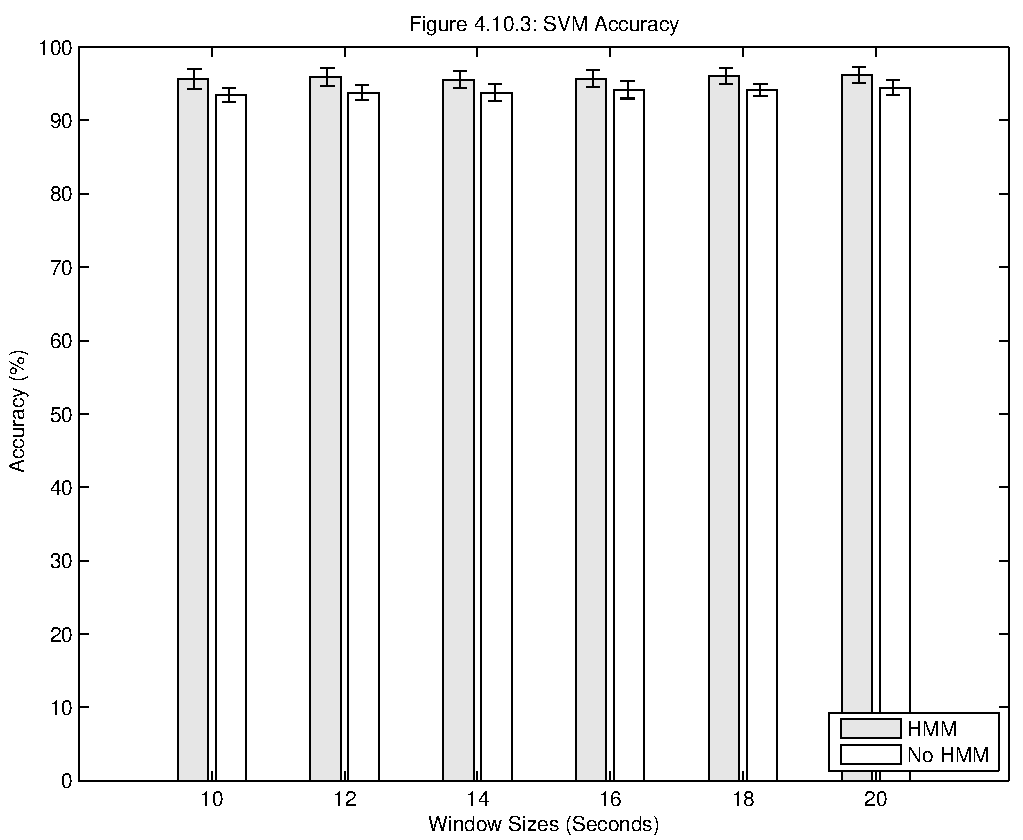
\includegraphics[scale=0.4]{osu_svm_hmm_nohmm_compare_acc.pdf} \hspace{1em}\vspace{1em}
 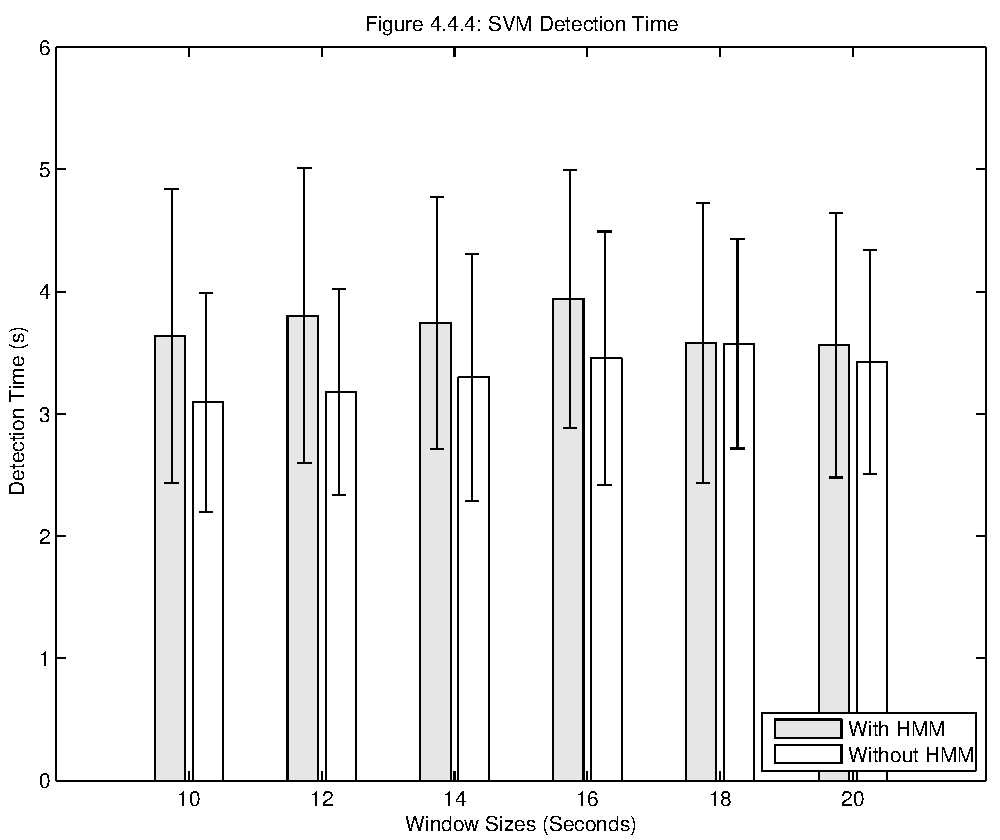
\includegraphics[scale=0.4]{osu_svm_hmm_nohmm_compare_det.pdf}
 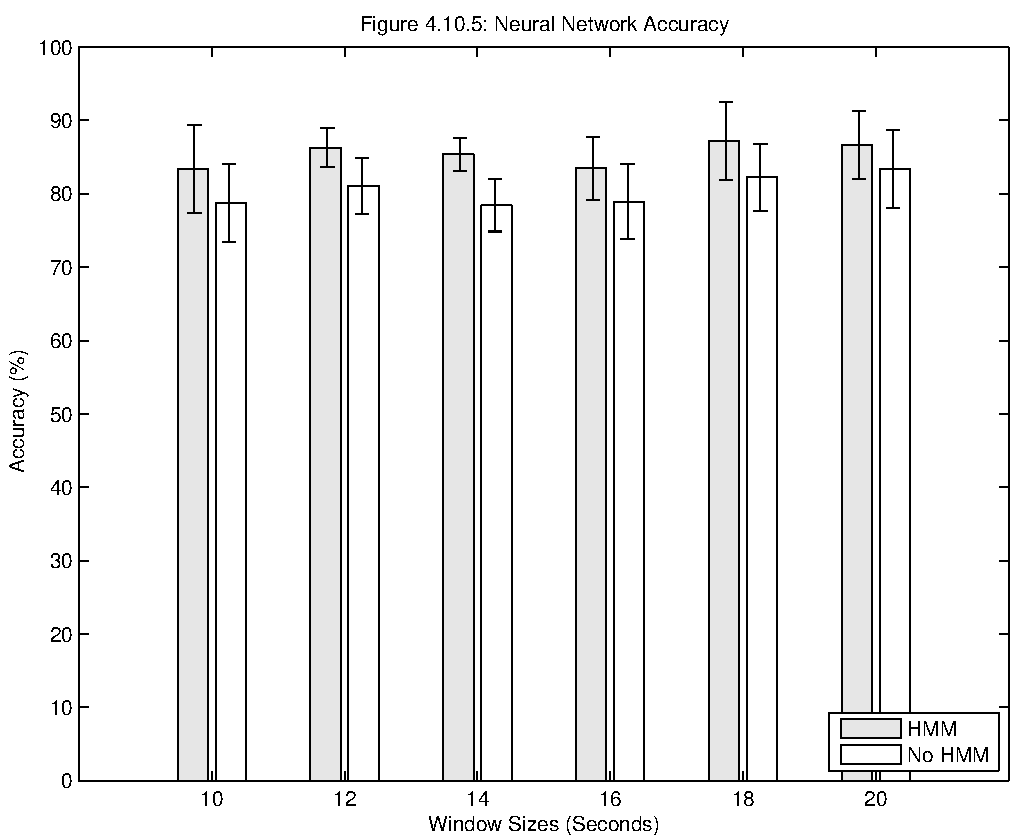
\includegraphics[scale=0.4]{osu_nnet_hmm_nohmm_compare_acc.pdf} \hspace{1em}
 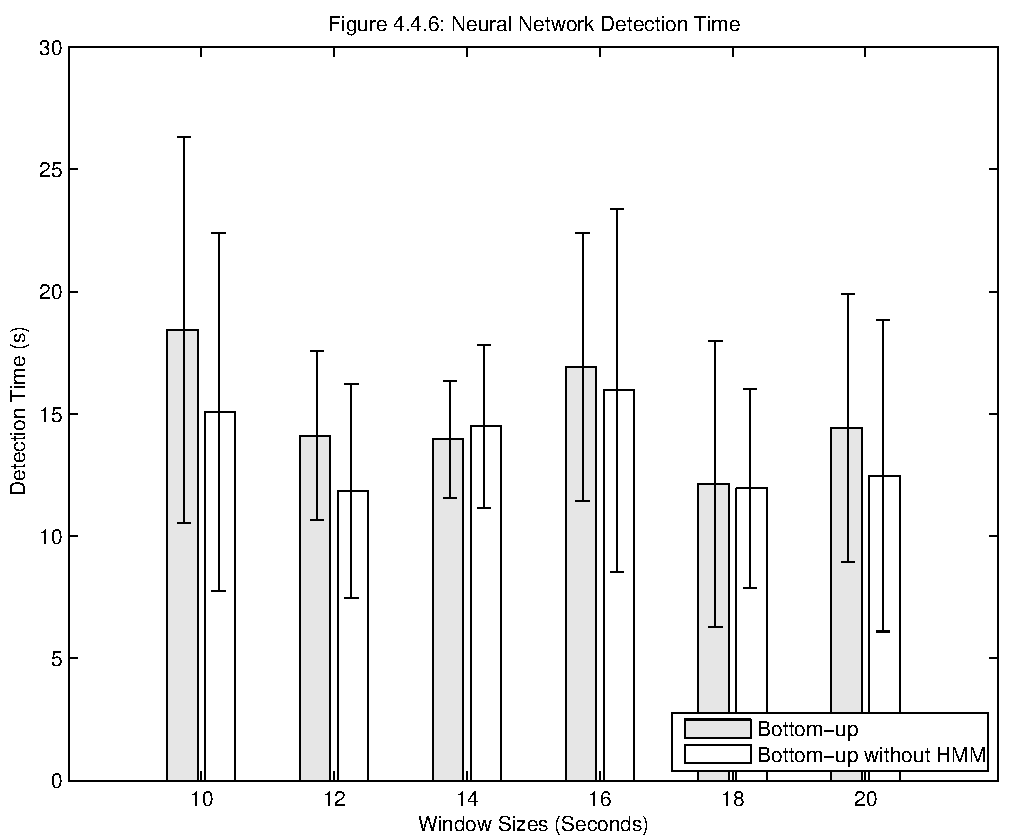
\includegraphics[scale=0.4]{osu_nnet_hmm_nohmm_compare_det.pdf}
 \caption{OSU Hip Results. Comparison of base classifier performance with and without the HMM
  smoothing layer, with test data split into fixed window sizes. Graphs are organized into rows by base
  classifier, and columns by evaluation metric. Error bars show a 95\% confidence interval.}
 \label{fig:osu_hmm}
\end{figure}

\begin{figure}[H]
 \centering
 %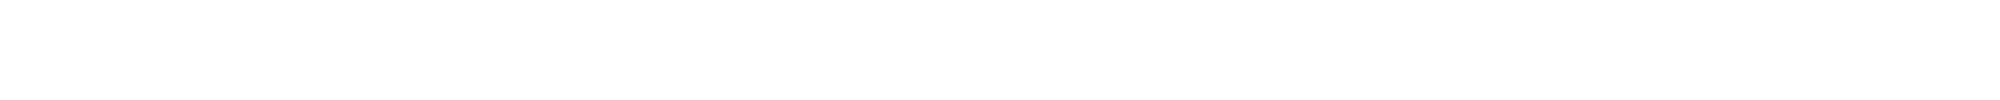
\includegraphics[scale=0.3]{vspace.png}
 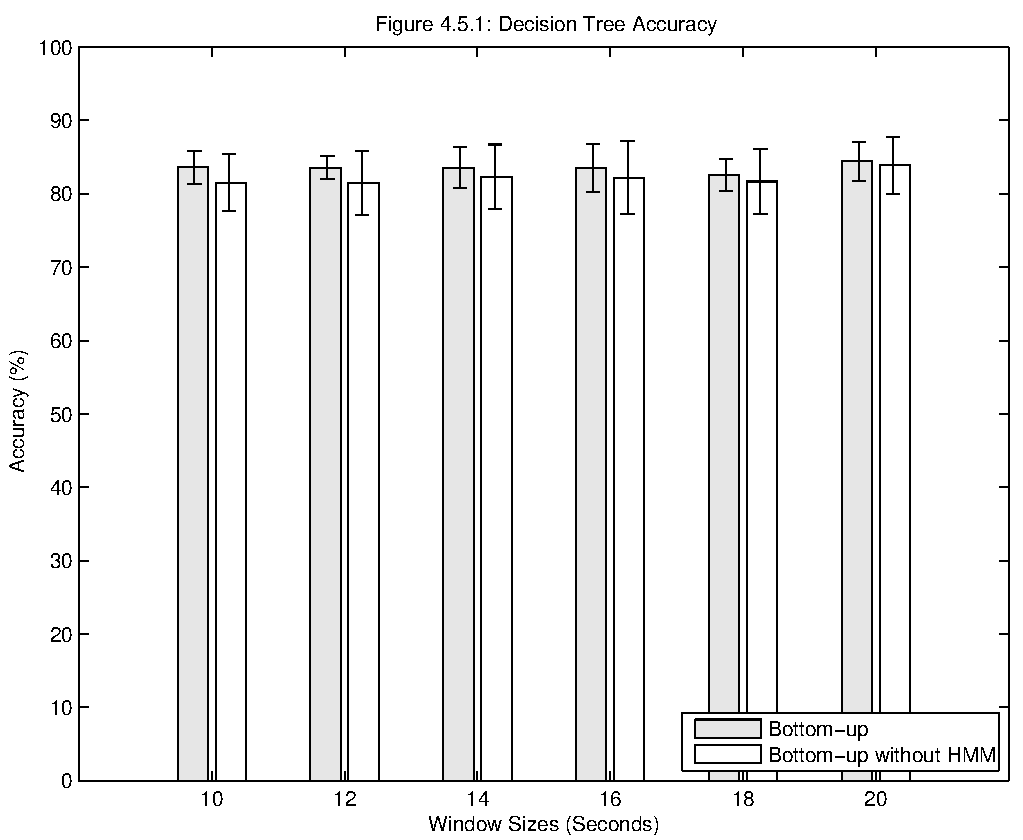
\includegraphics[scale=0.4]{lime1_dt_hmm_nohmm_compare_acc.pdf} \hspace{1em}\vspace{1em}
 \includegraphics[scale=0.4]{lime1_dt_hmm_nohmm_compare_det.pdf} 
 \includegraphics[scale=0.4]{lime1_svm_hmm_nohmm_compare_acc.pdf} \hspace{1em}\vspace{1em}
 \includegraphics[scale=0.4]{lime1_svm_hmm_nohmm_compare_det.pdf}
 \includegraphics[scale=0.4]{lime1_nnet_hmm_nohmm_compare_acc.pdf} \hspace{1em}
 \includegraphics[scale=0.4]{lime1_nnet_hmm_nohmm_compare_det.pdf}
 \caption{LiME Day 1 Results. Comparison of base classifier performance with and without the HMM
  smoothing layer, with test data split into fixed window sizes. Graphs are organized into rows by base
  classifier, and columns by evaluation metric. Error bars show a 95\% confidence interval.}
 \label{fig:lime1_hmm}
\end{figure}

\begin{figure}[H]
 \centering
 %\includegraphics[scale=0.3]{vspace.png}
 \includegraphics[scale=0.4]{lime2_dt_hmm_nohmm_compare_acc.pdf} \hspace{1em}\vspace{1em}
 \includegraphics[scale=0.4]{lime2_dt_hmm_nohmm_compare_det.pdf} 
 \includegraphics[scale=0.4]{lime2_svm_hmm_nohmm_compare_acc.pdf} \hspace{1em}\vspace{1em}
 \includegraphics[scale=0.4]{lime2_svm_hmm_nohmm_compare_det.pdf}
 \includegraphics[scale=0.4]{lime2_nnet_hmm_nohmm_compare_acc.pdf} \hspace{1em}
 \includegraphics[scale=0.4]{lime2_nnet_hmm_nohmm_compare_det.pdf}
 \caption{LiME Day 2 Results. Comparison of base classifier performance with and without the HMM
  smoothing layer, with test data split into fixed window sizes. Graphs are organized into rows by base
  classifier, and columns by evaluation metric. Error bars show a 95\% confidence interval.}
 \label{fig:lime2_hmm}
\end{figure}

%\begin{figure}[H]
% \centering
% \includegraphics[scale=0.4]{osu_hmm_dt_acc.pdf} \hspace{1em}\vspace{1em}
% \includegraphics[scale=0.4]{osu_hmm_dt_det.pdf}
% \includegraphics[scale=0.4]{osu_hmm_svm_acc.pdf} \hspace{1em}\vspace{1em}
% \includegraphics[scale=0.4]{osu_hmm_svm_det.pdf}
% \includegraphics[scale=0.4]{osu_hmm_nnet_acc.pdf} \hspace{1em}
% \includegraphics[scale=0.4]{osu_hmm_nnet_det.pdf}
% \caption{OSU Hip HMM Results.
%  Graphs are organized into rows by base classifier, and columns by evaluation
%  metric. HMM results were averaged over 10 splits into training
%  (base classifier), validation, training (HMM), and testing datasets. Error
%  bars show a 95\% confidence interval around the average.}
% \label{fig:osu_hmm}
%\end{figure}

%\begin{figure}[H]
% \centering
% \includegraphics[scale=0.4]{lime1_hmm_dt_acc.pdf} \hspace{1em}\vspace{1em}
% \includegraphics[scale=0.4]{lime1_hmm_dt_det.pdf} 
% \includegraphics[scale=0.4]{lime1_hmm_svm_acc.pdf} \hspace{1em}\vspace{1em}
% \includegraphics[scale=0.4]{lime1_hmm_svm_det.pdf} 
% \includegraphics[scale=0.4]{lime1_hmm_nnet_acc.pdf} \hspace{1em}
% \includegraphics[scale=0.4]{lime1_hmm_nnet_det.pdf} 
% \caption{LiME Day 1 HMM Results.
%  Graphs are organized into rows by base classifier, and columns by evaluation
%  metric. HMM results were averaged over 10 splits into training
%  (base classifier), validation, training (HMM), and testing datasets. Error
%  bars show a 95\% confidence interval around the average.}
% \label{fig:lime1_hmm}
%\end{figure}

%\begin{figure}[H]
% \centering
% \includegraphics[scale=0.4]{lime2_hmm_dt_acc.pdf} \hspace{1em}\vspace{1em}
% \includegraphics[scale=0.4]{lime2_hmm_dt_det.pdf}
% \includegraphics[scale=0.4]{lime2_hmm_svm_acc.pdf} \hspace{1em}\vspace{1em}
% \includegraphics[scale=0.4]{lime2_hmm_svm_det.pdf}
% \includegraphics[scale=0.4]{lime2_hmm_nnet_acc.pdf} \hspace{1em}
% \includegraphics[scale=0.4]{lime2_hmm_nnet_det.pdf}
% \caption{LiME Day 2 HMM Results.
%  Graphs are organized into rows by base classifier, and columns by evaluation
%  metric. HMM results were averaged over 10 splits into training
%  (base classifier), validation, training (HMM), and testing datasets. Error
%  bars show a 95\% confidence interval around the average.}
% \label{fig:lime2_hmm}
%\end{figure}

\newpage

\section{Discussion}

We found it difficult to directly compare performance between the
top-down and bottom-up approaches, because we
varied false positives per second in the top-down experiments,
and varied the fixed-length window size in the bottom-up experiments.
However, for a given false positive rate change-point
detection algorithms split a time series into windows of a certain average size,
which generally decreases as the false positive rate increases. From this it is possible
to relate false positive rates from the top-down experiments to
the window sizes of the bottom-up experiments. HMM false positive rates per second of
\{0.033, 0.028, 0.024, 0.021, 0.019, 0.017\} correspond to average
window sizes of \{10, 12, 14, 16, 18, 20\}. Figures \ref{fig:osu_compare_cpd_hmm},
\ref{fig:lime1_compare_cpd_hmm}, and \ref{fig:lime2_compare_cpd_hmm}
show a side-by-side comparison of the top-down and bottom-up approaches, using
this conversion. As seen in Section \ref{sec:cpd_results}, two algorithms 
were tested for each of the change-point detection experiments, but only the
best performing algorithm (highest in accuracy or lowest in detection time) is 
shown here, for each individual experiment.
Our results show that the bottom-up approach outperformed the top-down
approach, both in terms of accuracy
and detection time, regardless of the dataset and base classifier.

A contributing factor to the particularly high accuracy and low detection time
results generally attained for the OSU Hip experiments was that the data
consisted of activities that were synthetically glued together. The same group
of activities were performed in the same order by each of the 50 subjects in
this dataset, making transitions from one activity to the other very predictable
for a temporal model. By contrast, the LiME datasets consisted of unsynthetic
data gathered from a large set of unstructured and variable-length activities,
so the activity transitions were not as predictable and are more indicative of
an application of our techniques in the real world.

A final point of interest was that SVM (Figures 4.7.3, 4.7.4, 4.8.3, 4.8.4, 4.9.3, 4.9.4) clearly outperformed the other two
base classifiers, and that the faster and simpler decision tree model (Figures 4.7.1, 4.7.2, 4.8.1, 4.8.2, 4.9.1, 4.9.2) matched up
well against neural networks (Figures 4.7.5, 4.7.6, 4.8.5, 4.8.6, 4.9.5, 4.9.6). This result is significant because much of the
previous research that has formulated activity detection as a supervised learning
problem has used neural networks exclusively.

\begin{figure}[h]
 \centering
 %\includegraphics[scale=0.3]{vspace.png}
 \includegraphics[scale=0.4]{osu_dt_cpd_hmm_compare_acc_line.pdf} \hspace{1em}\vspace{1em}
 \includegraphics[scale=0.4]{osu_dt_cpd_hmm_compare_det_line.pdf} 
 \includegraphics[scale=0.4]{osu_svm_cpd_hmm_compare_acc_line.pdf} \hspace{1em}\vspace{1em}
 \includegraphics[scale=0.4]{osu_svm_cpd_hmm_compare_det_line.pdf}
 \includegraphics[scale=0.4]{osu_nnet_cpd_hmm_compare_acc_line.pdf} \hspace{1em}
 \includegraphics[scale=0.4]{osu_nnet_cpd_hmm_compare_det_line.pdf}
 \caption{Comparison of top-down and bottom-up results for OSU Hip.
  Graphs are organized into rows by base classifier, and columns by evaluation
  metric. Results for false positives per second of \{0.005, 0.01, 0.017, 0.019, 0.021, 0.024, 0.028, 0.033, 0.05, 0.1\} are 
  top-down experiments, while results for false positives per second of
  \{0.017, 0.019, 0.021, 0.024, 0.028, 0.033\} are bottom-up experiments.}
 \label{fig:osu_compare_cpd_hmm}
\end{figure}

\begin{figure}[h]
 \centering
 %\includegraphics[scale=0.3]{vspace.png}
 \includegraphics[scale=0.4]{lime1_dt_cpd_hmm_compare_acc_line.pdf} \hspace{1em}\vspace{1em}
 \includegraphics[scale=0.4]{lime1_dt_cpd_hmm_compare_det_line.pdf} 
 \includegraphics[scale=0.4]{lime1_svm_cpd_hmm_compare_acc_line.pdf} \hspace{1em}\vspace{1em}
 \includegraphics[scale=0.4]{lime1_svm_cpd_hmm_compare_det_line.pdf}
 \includegraphics[scale=0.4]{lime1_nnet_cpd_hmm_compare_acc_line.pdf} \hspace{1em}
 \includegraphics[scale=0.4]{lime1_nnet_cpd_hmm_compare_det_line.pdf}
 \caption{Comparison of top-down and bottom-up results for LiME Day 1.
  Graphs are organized into rows by base classifier, and columns by evaluation
  metric. Results for false positives per second of \{0.005, 0.01, 0.05, 0.1\} are
  top-down experiments, while results for false positives per second of
  \{0.017, 0.019, 0.021, 0.024, 0.028, 0.033\} are bottom-up experiments.}
 \label{fig:lime1_compare_cpd_hmm}
\end{figure}

\begin{figure}[h]
 \centering
 %\includegraphics[scale=0.3]{vspace.png}
 \includegraphics[scale=0.4]{lime2_dt_cpd_hmm_compare_acc_line.pdf} \hspace{1em}\vspace{1em}
 \includegraphics[scale=0.4]{lime2_dt_cpd_hmm_compare_det_line.pdf} 
 \includegraphics[scale=0.4]{lime2_svm_cpd_hmm_compare_acc_line.pdf} \hspace{1em}\vspace{1em}
 \includegraphics[scale=0.4]{lime2_svm_cpd_hmm_compare_det_line.pdf}
 \includegraphics[scale=0.4]{lime2_nnet_cpd_hmm_compare_acc_line.pdf} \hspace{1em}
 \includegraphics[scale=0.4]{lime2_nnet_cpd_hmm_compare_det_line.pdf}
 \caption{Comparison of top-down and bottom-up results for LiME Day 2.
  Graphs are organized into rows by base classifier, and columns by evaluation
  metric. Results for false positives per second of \{0.005, 0.01, 0.05, 0.1\} are
  top-down experiments, while results for false positives per second of
  \{0.017, 0.019, 0.021, 0.024, 0.028, 0.033\} are bottom-up experiments.}
 \label{fig:lime2_compare_cpd_hmm}
\end{figure}

\section{Timing}

Since we are interested in the feasibility of performing activity detection on
accelerometer data in real time, we tested how long it would require our
approaches to segment and classify a time series in a streaming, online fashion.
Experiments were performed using an Intel(R) Core(TM) 2 Quad Processor Q9550.

There are three different computations that a device must perform to do
activity recognition in real time. The first (when using the top-down approach)
is to calculate a change-point
detection score for an individual time tick. When the device obtains a new tick of
accelerometer data, it must generate a change-point detection score and compare
it to the score threshold to decide whether or not to predict an activity
change. We estimated the amount of time required to determine whether an
activity change should be predicted by choosing 1000 random ticks from our data,
and running our two change-point detection algorithms on the reference and test
data corresponding to each tick. We found that on average the control chart algorithm
took 0.050ms per tick, and that the KLIEP algorithm took 31.4ms per tick. If no change
was predicted, then the device needs to take no further action for this tick.

If a change was predicted in the first step, then the second step is to
featurize the window of data corresponding to the activity that just ended.
The amount of time required to featurize an activity window increases with the
length of the window. The OSU Hip dataset contained 120 second long activities,
and the median length of the LiME activities was considerably smaller than that,
therefore we fixed the window length at 120 seconds for this experiment. The
amount of time required to featurize these windows, again averaged over 1000 runs,
was 98.5ms.

Once the data from an activity window is featurized, the activity must be
predicted using a base classifier. We assume that the classifier has already
been trained and validated previously. We averaged the activity prediction time
over 60 runs on each of our base classifiers, with featurized windows and models
built during our change-point detection experiments. We found that the average
time required to predict an activity with decision trees was 372ms, with
SVMs was 368ms, and with neural networks was 369ms.

These experiments show that the amount of time required to process an activity
tick when a change is predicted is in the worst case
31.4ms + 98.5ms + 372ms = 501ms, which is a very reasonable amount of time
for an online application.

\chapter{Conclusion}
The purpose of this work was to test the feasibility of classifying 
accelerometer data in real time. We were also interested in using change-point
detection techniques for deciding when one activity ended within a time series
and the next began, and to contrast this methodology with an HMM approach.
The bottom-up approach clearly outperformed the top-down approach in terms
of both accuracy and detection time, because our change-point detection
algorithms did a poor job of correctly classifying the data, and because the
HMM temporal model is very well-suited to time series data.


\bibliographystyle{plain}
\bibliography{thesis}

%\appendix
%\chapter{Redundancy}
%This appendix is inoperable.
%
\end{document}
